%File: anonymous-submission-latex-2025.tex
\documentclass[letterpaper]{article}
\usepackage{aaai25}
\usepackage{graphicx}
\usepackage{times}  % DO NOT CHANGE THIS
\usepackage{helvet}  % DO NOT CHANGE THIS
\usepackage{courier}  % DO NOT CHANGE THIS
\usepackage[hyphens]{url}  % DO NOT CHANGE THIS
\usepackage{graphicx} % DO NOT CHANGE THIS
\usepackage{tabularx} % DO NOT CHANGE THIS
\usepackage{supertabular} % DO NOT CHANGE THIS
\usepackage{booktabs}
\usepackage{arabtex}
\usepackage{utf8}
\setcode{utf8}
\usepackage{tcolorbox}

\usepackage[utf8]{inputenc}



\urlstyle{rm} % DO NOT CHANGE THIS
\def\UrlFont{\rm}  % DO NOT CHANGE THIS
\usepackage{natbib}  % DO NOT CHANGE THIS AND DO NOT ADD ANY OPTIONS TO IT
\usepackage{caption} % DO NOT CHANGE THIS AND DO NOT ADD ANY OPTIONS TO IT
\frenchspacing  % DO NOT CHANGE THIS
\setlength{\pdfpagewidth}{8.5in} % DO NOT CHANGE THIS
\setlength{\pdfpageheight}{11in} % DO NOT CHANGE THIS
%
% These are recommended to typeset algorithms but not required. See the subsubsection on algorithms. Remove them if you don't have algorithms in your paper.
\usepackage{algorithm}
\usepackage{algorithmic}

%
% These are are recommended to typeset listings but not required. See the subsubsection on listing. Remove this block if you don't have listings in your paper.
\usepackage{newfloat}
\usepackage{listings}
\DeclareCaptionStyle{ruled}{labelfont=normalfont,labelsep=colon,strut=off} % DO NOT CHANGE THIS
\lstset{%
	basicstyle={\footnotesize\ttfamily},% footnotesize acceptable for monospace
	numbers=left,numberstyle=\footnotesize,xleftmargin=2em,% show line numbers, remove this entire line if you don't want the numbers.
	aboveskip=0pt,belowskip=0pt,%
	showstringspaces=false,tabsize=2,breaklines=true}
\floatstyle{ruled}
\newfloat{listing}{tb}{lst}{}
\floatname{listing}{Listing}
%
% Keep the \pdfinfo as shown here. There's no need
% for you to add the /Title and /Author tags.
\pdfinfo{
/TemplateVersion (2025.1)
}

% DISALLOWED PACKAGES
% \usepackage{authblk} -- This package is specifically forbidden
% \usepackage{balance} -- This package is specifically forbidden
% \usepackage{color (if used in text)
% \usepackage{CJK} -- This package is specifically forbidden
% \usepackage{float} -- This package is specifically forbidden
% \usepackage{flushend} -- This package is specifically forbidden
% \usepackage{fontenc} -- This package is specifically forbidden
% \usepackage{fullpage} -- This package is specifically forbidden
% \usepackage{geometry} -- This package is specifically forbidden
% \usepackage{grffile} -- This package is specifically forbidden
% \usepackage{hyperref} -- This package is specifically forbidden
% \usepackage{navigator} -- This package is specifically forbidden
% (or any other package that embeds links such as navigator or hyperref)
% \indentfirst} -- This package is specifically forbidden
% \layout} -- This package is specifically forbidden
% \multicol} -- This package is specifically forbidden
% \nameref} -- This package is specifically forbidden
% \usepackage{savetrees} -- This package is specifically forbidden
% \usepackage{setspace} -- This package is specifically forbidden
% \usepackage{stfloats} -- This package is specifically forbidden
% \usepackage{tabu} -- This package is specifically forbidden
% \usepackage{titlesec} -- This package is specifically forbidden
% \usepackage{tocbibind} -- This package is specifically forbidden
% \usepackage{ulem} -- This package is specifically forbidden
% \usepackage{wrapfig} -- This package is specifically forbidden
% DISALLOWED COMMANDS
% \nocopyright -- Your paper will not be published if you use this command
% \addtolength -- This command may not be used
% \balance -- This command may not be used
% \baselinestretch -- Your paper will not be published if you use this command
% \clearpage -- No page breaks of any kind may be used for the final version of your paper
% \columnsep -- This command may not be used
% \newpage -- No page breaks of any kind may be used for the final version of your paper
% \pagebreak -- No page breaks of any kind may be used for the final version of your paperr
% \pagestyle -- This command may not be used
% \tiny -- This is not an acceptable font size.
% \vspace{- -- No negative value may be used in proximity of a caption, figure, table, section, subsection, subsubsection, or reference
% \vskip{- -- No negative value may be used to alter spacing above or below a caption, figure, table, section, subsection, subsubsection, or reference

\setcounter{secnumdepth}{0} %May be changed to 1 or 2 if section numbers are desired.

% The file aaai25.sty is the style file for AAAI Press
% proceedings, working notes, and technical reports.
%

% Title

% Your title must be in mixed case, not sentence case.
% That means all verbs (including short verbs like be, is, using,and go),
% nouns, adverbs, adjectives should be capitalized, including both words in hyphenated terms, while
% articles, conjunctions, and prepositions are lower case unless they
% directly follow a colon or long dash
\title{Sacred or Synthetic? Evaluating LLM Reliability and Abstention for Religious Questions}

\author {
    Farah Atif\textsuperscript{\rm 1},
    Nursultan Askarbekuly\textsuperscript{\rm 2}, 
    Kareem Darwish\textsuperscript{\rm 3},
    Monojit Choudhury\textsuperscript{\rm 1}
}
\affiliations {
    \textsuperscript{\rm 1}Mohamed Bin Zayed University of AI\\
    \textsuperscript{\rm 2}Innopolis University\\
    \textsuperscript{\rm 3}Hamad Bin Khalifa University\\
    farah.atif@mbzuai.ac.ae, n.askarbekuly@innopolis.university, 
    kadarwish@hbku.edu.qa, monojit.choudhury@mbzuai.ac.ae	
}

%Example, Single Author, ->> remove \iffalse,\fi and place them surrounding AAAI title to use it
\iffalse
\title{My Publication Title --- Single Author}
\author {
    Author Name
}
\affiliations{
    Affiliation\\
    Affiliation Line 2\\
    name@example.com
}
\fi

\iffalse
%Example, Multiple Authors, ->> remove \iffalse,\fi and place them surrounding AAAI title to use it
\title{My Publication Title --- Multiple Authors}
\author {
    % Authors
    First Author Name\textsuperscript{\rm 1},
    Second Author Name\textsuperscript{\rm 2},
    Third Author Name\textsuperscript{\rm 1}
}
\affiliations {
    % Affiliations
    \textsuperscript{\rm 1}Affiliation 1\\
    \textsuperscript{\rm 2}Affiliation 2\\
    firstAuthor@affiliation1.com, secondAuthor@affilation2.com, thirdAuthor@affiliation1.com
}
\fi


% REMOVE THIS: bibentry
% This is only needed to show inline citations in the guidelines document. You should not need it and can safely delete it.
\usepackage{bibentry}
% END REMOVE bibentry

\begin{document}


\maketitle

\begin{abstract}

% Despite the increasing usage of Large Language Models (LLMs) in answering in questions in a variety of domains, their reliability and accuracy remain largely unexamined for some domains including the religious domain. In this paper, we address the lack of rigorous evaluation and ethical oversight in this context by introducing a novel benchmark \textit{IlmQuest} focused on Islamic rulings explicitly categorized by the four major Sunni schools of thought, in both Arabic and English. Unlike prior work, which either overlooks legal school distinctions or fails to evaluate abstention behavior, we assess LLMs not only on their accuracy but also on their ability to recognize when not to answer. Our zero-shot and abstention experiments reveal significant variation across models, languages, and legal schools. While GPT-4o outperforms all other models in accuracy, Gemini and Fanar demonstrate superior abstention behavior critical for minimizing confident incorrect answers. Notably, all models exhibit a performance drop in Arabic, highlighting the limitations in religious reasoning for languages other than English. To the best of our knowledge, this is the first study to evaluate LLM abstention for religion-based factual queries. Our findings underscore the need for culturally grounded evaluation and cautious deployment of LLMs in religious applications.
Despite the increasing usage of Large Language Models (LLMs) in answering questions in a variety of domains, their reliability and accuracy remain unexamined for a plethora of domains including the religious domains. In this paper, we introduce a novel benchmark \textit{FiqhQA} \footnote{https://huggingface.co/datasets/MBZUAI/FiqhQA} focused on the LLM generated Islamic rulings explicitly categorized by the four major Sunni schools of thought, in both Arabic and English. Unlike prior work, which either overlooks the distinctions between religious school of thought or fails to evaluate abstention behavior, we assess LLMs not only on their accuracy but also on their ability to recognize when not to answer. Our zero-shot and abstention experiments reveal significant variation across LLMs, languages, and legal schools of thought. While GPT-4o outperforms all other models in accuracy, Gemini and Fanar demonstrate superior abstention behavior critical for minimizing confident incorrect answers. Notably, all models exhibit a performance drop in Arabic, highlighting the limitations in religious reasoning for languages other than English. To the best of our knowledge, this is the first study to benchmark the efficacy of LLMs for fine-grained Islamic school of thought specific ruling generation and to evaluate abstention for Islamic jurisprudence queries. Our findings underscore the need for task-specific evaluation and cautious deployment of LLMs in religious applications.
\end{quote}
\end{abstract}

% Uncomment the following to link to your code, datasets, an extended version or similar.
%
% \begin{links}
%     \link{Code}{https://aaai.org/example/code}
%     \link{Datasets}{https://aaai.org/example/datasets}
%     \link{Extended version}{https://aaai.org/example/extended-version}
% \end{links}

\section{Introduction}
With the rapid advancement of Large Language Models (LLMs), chat systems have witnessed unprecedented adoption. These systems can address a wide range of tasks and can answer questions across various domains. However, their reliability remains questionable, particularly when models exhibit uncertainty in their responses. This uncertainty poses serious risks, especially in sensitive high-stakes domains such as medicine, military affairs, religion, and ethics \cite{madhusudhan2024llms,lin2021truthfulqa}.

% people ask LLMs
% the need to answer accurately and be aware of the four schools of law
% With increasing LLM adoption, 
In fact, many users now turn to LLMs for religious guidance, including questions about Islamic law and practice. Traditionally, rulings or Fatwas are issued by trained scholars through a rigorous process typically grounded within an Islamic jurisprudence school of thought, i.e. a madhhab. For the four main Sunni schools of thought, namely Hanafi, Maliki, Shafi‘i, and Hanbali, each derives rulings based on distinct legal methodologies that provide authenticity and consistency. Scholars are trained within these schools, and many online platforms (e.g., IslamQA.org) present rulings accordingly, recognizing their differences. Given this context, it is essential that LLMs answer Islamic questions accurately and with awareness of the jurisprudential schools of thought. Religious responses must therefore be both reliable and sensitive to the diversity within Islamic jurisprudence.

Several efforts have been made to develop Islamic Question Answering (QA) systems, benchmarks, and automated QA solutions. However, these approaches come with notable limitations. First, many existing QA datasets categorize questions by topic, yet, to the best of our knowledge, none have considered classification based on the four schools of thought.  This is despite the fact that they are widely followed by Sunni Muslims, with their adoption varying by region. Therefore, incorporating this categorization into benchmarks is crucial.

Second, while most previous studies have focused on fine-tuning models for Islamic QA, limited work has been done to assess LLMs in terms of their ability to answer religious questions accurately and abstain from answering when unsure. Abstention is critical given that there is a risk of LLM hallucinations, even with Retrieval-Augmented Generation (RAG) \cite{niu2023ragtruth, song2024rag}. In other words, similar to a human expert, an LLM should know when not to answer. 

Finally, the evaluation of these systems remains an open problem as there is no consensus on the approach or metrics to use. Many benchmarks use multiple-choice questions for the sake of simplicity \cite{koto2024arabicmmlu,rajpurkar2016squad}. However, the nature of our problem necessitates open-ended answers. For such cases, previous works often use some form of semantic distance \cite{zhong2022towards,zhang2019bertscore, yuan2021bartscore}, and more modern approaches utilize LLM-as-a-judge to evaluate answers \cite{kojima2022large,bai2024mt,liu2023g}. 

Within this work, we aim to investigate the extent to which LLMs can accurately answer religious questions according to a particular school of thought and whether they can recognize when they should abstain from responding. To this end, we address the following research questions:

\begin{itemize}
    \item To what extent are LLMs capable of answering religious questions?
    \item Can LLMs answer religious questions in accordance with a specific school of thought (madhhab)? 
    \item Does the language of the question affect the ability of LLMs to answer religious questions? 
    \item Do LLM's know when not to answer religious questions?
    
\end{itemize}

\noindent The contributions of this paper are as follows.
\begin{itemize}
%    \item To the best of our knowledge, this is the first paper to investigate LLM ability to provide madhhab answers and to abstain when not sure.
    \item We manually curate a dataset with 960 questions and answers for all four schools of thought, both in English and Arabic.
    \item We propose and employ a robust evaluation methodology that examines the accuracy of several LLMs when answering questions according to a school of thought and their ability to abstain from providing an answer when uncertain.
    % \item We evaluate several LLMs on their ability to provide madhhab specific answers and to abstain when uncertain.
\end{itemize}


\section{Related works}
Several studies have focused on question answering (QA) within the religious domain, particularly in the context of Islam. These works can be broadly categorized into three main areas: Qur’an QA, Hadith QA, and Fatwa QA.

The "Qur’an QA 2022" shared task \cite{malhas-etal-2023-quran} focused on extracting answers from the Qur’an that are relevant user queries. Similarly, previous studies have proposed QA corpora based on the Qur’an, including the works of \citet{abdelnasser2014bayan}, \citet{malhas2020ayatec}, and \citet{alqahtani2018annotated}. For Hadith-based QA, \citet{wiharja2022questions} introduced a Hadith knowledge graph to facilitate Islamic QA and proposed a reasoning mechanism. \citet{rizqullah2023qasina} developed a new Hadith QA dataset in the Indonesian language. The focus of the above works is specifically on one particular legal source, and do not allow for comprehensive question answering that incorporates both the sources and legal principles.

A different approach is that of \citet{qamar2024benchmark}, who gathered a QA dataset based on IslamQA.org portal, Quranic Tafsir (Quran commentary), and Ahadith. They then finetuned several language models and evaluated each model's answers in terms of the ability to understand the question and answer it accurately. \citet{mohammed2022english} also composed a dataset by parsing several sources, then labeling and categorizing them. The idea behind such datasets is to facilitate retrieval-augmented generation (RAG).

More recently, \citet{patel2023building} compared GPT-3.5 and GPT-4 in answering Islamic questions using several basic prompting techniques. They also experimented with RAG and finetuning for GPT-3.5, then evaluated using BERTScore and embedding distance.

Most of these papers are reporting challenges related to accuracy of answers. Yet none of them address the issue of abstention, i.e. the ability to not answer when unsure. Abstention is an active area of LLM-related research \cite{kasai2023realtime,rottger-etal-2024-xstest,ahdritz2024distinguishing,kim2024epistemology,madhusudhan2024llms} and is central to Islamic tradition. A popular proverb among jurists states: "Whomsoever says: `I don't know' has amassed half of knowledge." % : a famous story  describes Imam Malik being asked by a person who traveled for six months to ask a question, and his answer was \textit{I don't know} \cite{ibnAbdAlBarr1994}.

Another aspect that the existing research does not address is the issue of schools of legal thought (madhhabs). In practice, human jurists are trained within the framework of specific schools and answer accordingly. 

Lastly, the existing evaluation methodologies in Islamic QA research use BERTScore, ROUGE, and embedding distance as evaluation metrics. These can be expanded by newer evaluation techniques such as LLM-as-a-judge with cross-checked human annotation.
% and Krippendorff's alpha score to balance reliability and efficiency.


% Alternative name: madhhabsLLM?
\section{FiqhQA Dataset}
\label{sec:dataset}

The goal of this study is to evaluate whether LLMs can answer religious questions from the perspective of Islamic jurisprudence schools of thought, i.e. be able to navigate the commonalities and differences between the schools of thought and provide correct answers in accordance with each school. To achieve this goal, we propose the construction of a dataset, FiqhQA, that explicitly categorizes Islamic rulings according to the four major Sunni schools of thought, namely Maliki, Shafi'i, Hanafi, and Hanbali. The dataset is further organized into thematic categories such as Prayer, Fasting, Purity, Marriage and Divorce, Charity, and Pilgrimage. In this study, we focus specifically on rulings, i.e. the established legal positions of each of the schools, as opposed to fatwas which are inherently more specific and flexible to the context at hand. 

% First, our examination of various fatwa portals revealed significant variability in responses across scholars. Some scholars provide detailed justifications from the Qur'an and Sunnah, resulting in a broader and more diverse answer space, while others offer concise responses without explicit references. Second, fatwas are often personalized, taking into account the specific circumstances of the individual posing the question. This personalization introduces an additional layer of complexity in terms of interpretation and evaluation.

% In contrast, rulings are generally more standardized, with well-defined answers that do not require personalization. Moreover, it is comparatively easier to retrieve consistent rulings across all four schools of thought. For these reasons, our work focuses on factoid-style questions derived from rulings, ensuring greater consistency and clarity in the dataset.

\subsection{Dataset construction} We chose Kuwaiti Fiqh Encyclopedia\footnote{https://muslim-library.com/keoj/} as the primary source, as it is a well-established and is an authoritative reference extensively covering the legal rulings (ahkam) across the four Sunni madhhabs. The encyclopedia is systematically organized by topic and terminology, and has a clear presentation of the differing positions among the schools, making it particularly well suited for dataset construction.

\subsection{Scope and Category Selection}
The dataset centers on rulings within the domain of Fiqh al-'Ibadat, which are acts of worship and ritual obligations. The inclusion criteria were developed in consultation with a domain expert. For Fiqh al-'Ibadat, relevant rulings were manually extracted based on a set of predefined conceptual categories. Each entry was then annotated with the specific positions held by the respective schools, reflecting their unique methodologies and legal interpretations.

% In contrast, for \textit{Fiqh al-Mu’amalat}, the modern scholarly approach often consolidates rulings into standardized frameworks, such as those proposed by AAOIFI (Accounting and Auditing Organization for Islamic Financial Institutions). For \textit{‘Aqeedah}, the dataset follows the mainstream doctrines of Ahlus-Sunnah wa'l-Jama'ah, while avoiding contentious issues related to the mutashabihat, where significant differences exist between Salafi and traditional theological schools.

The categories selected for the current stage of dataset development are as follows:
\begin{itemize}
    \item Prayer (Salat)
    \item Fasting (Sawm)
    \item Purification (Taharah)
    \item Marriage and divorce
    \item Almsgiving (Zakat and Sadaqah)
    \item Pilgrimage (Hajj and ‘Umrah)
\end{itemize}

Following the extraction of rulings, we employed GPT-4o to generate corresponding question–answer pairs for each ruling. Since the original source is in Arabic, all generated content was reviewed and validated by native Arabic speakers. For the English version of the dataset, the Arabic question–answer pairs were translated using GPT-4o, with subsequent manual verification by human annotators to ensure accuracy and fidelity.

In several instances, generated questions required manual refinement, particularly when the initial phrasing allowed for overly broad answers. Translations of both questions and answers were also manually checked and corrected, where necessary, to maintain clarity and precision across languages.

In total, the dataset consists of 960 question-answer pairs. These are based on 120 unique questions, each available in both Arabic and English, with four answers corresponding to the four schools of thought (120 questions x 2 languages x 4 schools of thought = 960). %, and for every question, four answers—corresponding to the Hanafi, Maliki, Shafi‘i, and Hanbali schools—are provided in both languages (240*4=960).
Figure \ref{fig:example-question} shows one of the question-answer pairs. 

% \begin{figure}[h]
%     \centering
%     \begin{minipage}[b]{0.48\textwidth}
%     \centering
%     \includegraphics[width=\textwidth,height=7cm]{AnonymousSubmission/LaTeX/sample2.png}
%     \caption{Example of English data}
%     \label{fig:sampledata}
%     \end{minipage}
% \end{figure}

\begin{figure}
    \centering
    \small
     \begin{tcolorbox}[colback=black!10, boxrule=0pt]
     {
\textbf{ID}: 05\\
\textbf{Agreement}: Disagreement\\
\textbf{Title}: Funeral Prayer for the Absent Person,\\
\textbf{Category}: Prayer,\\
\textbf{Statement}: Scholars have differed regarding the funeral prayer for an absent person. Abu Hanifa, Malik, and their followers held that it is not prescribed. Their response to the story of Najashi and the prayer offered for him is that this was a special privilege of the Prophet (peace and blessings be upon him). On the other hand, Al-Shafi'i, Ahmad, and their followers considered it to be prescribed, as it has been established through two authentic hadiths, and claiming it as a special privilege requires evidence.\\
\textbf{Question:} What is the ruling on performing the funeral prayer for the absent deceased?\\
\textbf{Maliki}: Malik held that the funeral prayer for an absent person is not prescribed. His response to the story of Najashi and the prayer offered for him is that this was a special privilege of the Prophet peace be upon him.\\
\textbf{Hanafi}: Abu Hanifa held that the funeral prayer for an absent person is not prescribed. His response to the story of Najashi and the prayer offered for him is that this was a special privilege of the Prophet peace be upon him.\\
\textbf{Shafi'i}: Al-Shafi'i considered the funeral prayer for an absent person to be prescribed, as it has been established through two authentic hadiths, and claiming it as a special privilege of the prophet requires evidence.\\
\textbf{Hanbali}: Imam Ahmad considered the funeral prayer for an absent person to be prescribed, as it has been established through two authentic hadiths, and claiming it as a special privilege requires evidence.
%     \\

% ``ID'': ``05'',\\
% ``Agreement": ``Disagreement'',\\
% ``Title": ``Funeral Prayer for the Absent Person'',\\
% ``Statement'': ``Scholars have differed regarding the funeral prayer for an absent person. Abu Hanifa, Malik, and their followers held that it is not prescribed. Their response to the story of Najashi and the prayer offered for him is that this was a special privilege of the Prophet ﷺ. On the other hand, Al-Shafi'i, Ahmad, and their followers considered it to be prescribed, as it has been established through two authentic hadiths, and claiming it as a special privilege requires evidence.''\\

% ``Question'': ``What is the ruling on performing the funeral prayer for the absent deceased?'',\\

% ``Maliki'': ``Malik held that the funeral prayer for an absent person is not prescribed. His response to the story of Najashi and the prayer offered for him is that this was a special privilege of the Prophet peace be upon him.''\\

% ``Hanafi'': ``Abu Hanifa held that the funeral prayer for an absent person is not prescribed. His response to the story of Najashi and the prayer offered for him is that this was a special privilege of the Prophet peace be upon him.'' \\

% ``Shafi'i'': ``Al-Shafi'i considered the funeral prayer for an absent person to be prescribed, as it has been established through two authentic hadiths, and claiming it as a special privilege of the prophet requires evidence.'',\\

% ``Hanbali'': ``Imam Ahmad considered the funeral prayer for an absent person to be prescribed, as it has been established through two authentic hadiths, and claiming it as a special privilege requires evidence.''
%      \\
    % "statement_ar": "\begin{RLtext}\<وَاخْتَلَفَ الْفُقَهَاءُ فِي الْمُدَّةِ الَّتِي يَجُوزُ تَعْجِيل الزَّكَاةِ فِيهَا: فَذَهَبَ الْحَنَفِيَّةُ: إِلَى جَوَازِ تَعْجِيل الزَّكَاةِ لِسِنِينَ، لِوُجُودِ سَبَبِ الْوُجُوبِ، وَهُوَ: مِلْكُ النِّصَابِ النَّامِي. وَقَيَّدَهُ الْحَنَابِلَةُ بِحَوْلَيْنِ فَقَطْ، اقْتِصَارًا عَلَى مَا وَرَدَ. فَقَدْ رَوَى عَلِيٌّ ﵁ أَنَّ النَّبِيَّ ﷺ تَعَجَّل مِنَ الْعَبَّاسِ ﵁ صَدَقَةَ سَنَتَيْنِ (١) لِقَوْلِهِ ﷺ: أَمَّا الْعَبَّاسُ فَهِيَ عَلَيَّ وَمِثْلُهَا مَعَهَا (٢) وَلِمَا رَوَى أَبُو دَاوُدَ مِنْ أَنَّ النَّبِيَّ ﷺ تَسَلَّفَ مِنَ الْعَبَّاسِ صَدَقَةَ عَامَيْنِ (٣) وَهُوَ وَجْهٌ عِنْدَ الشَّافِعِيَّةِ، صَحَّحَهُ الإِْسْنَوِيُّ وَغَيْرُهُ، وَعَزَوْهُ لِلنَّصِّ. وَذَهَبَ الشَّافِعِيَّةُ: إِلَى عَدَمِ جَوَازِ تَعْجِيل الزَّكَاةِ لأَِكْثَرَ مِنْ عَامٍ، وَذَلِكَ: لأَِنَّ زَكَاةَ غَيْرِ الْعَامِ الأَْوَّل لَمْ يَنْعَقِدْ حَوْلُهَا، وَالتَّعْجِيل قَبْل انْعِقَادِ الْحَوْل لاَ يَجُوزُ، كَالتَّعْجِيل قَبْل كَمَال النِّصَابِ فِي الزَّكَاةِ الْعَيْنِيَّةِ. أَمَّا الْمَالِكِيَّةُ: فَلَمْ يُجِيزُوا تَعْجِيل الزَّكَاةِ لأَِكْثَرَ مِنْ شَهْرٍ قَبْل الْحَوْل عَلَى الْمُعْتَمَدِ، وَتُكْرَهُ عِنْدَهُمْ بِشَهْرٍ>\end{RLtext}",
   
}
    \end{tcolorbox} 
    \caption{An example of English data, presenting a question and contrasting the viewpoints of the four major Sunni schools of thought.}
    \label{fig:example-question}
\end{figure}

\section{Experiment}
To ensure the rigor and reliability of our evaluation, we combined automated and human-driven procedures to evaluate LLM zero-shot QA capabilities and abstention. % Below we summarize the steps taken, the inter-annotator agreement computation, and additional considerations.

\subsection{Experimental Setup}
For zero-shot experiments, we evaluated LLMs on the full FiqhQA dataset using a zero-shot prompting strategy. For each of the 960 questions, %120 questions per madhhab in English and the same 120 question in Arabic (960 total), 
the model-generated answer was compared against the ground-truth answer. 

For abstention experiments, we evaluated the LLMs using 10\% of the questions in the FiqhQA dataset, which included 12 questions for each madhhab in both Arabic and English.  We augmented the questions with one of two abstention clauses variant, basic and strict (see figures \ref{fig:mesh1} and \ref{fig:mesh2}), as proposed by \citet{madhusudhan2024llms}.  The difference between the basic and strict prompts is that the strict one provides additional warnings to the LLM.  We further improved on the prompts of 
\citet{madhusudhan2024llms} as their original prompts resulted in weak abstention abilities.

\begin{figure}
    \centering
    \small
    \begin{tcolorbox}[colback=black!10, boxrule=0pt]
\{
    \\
    \hspace{0.5cm}"role": "system", \\
    \hspace{0.5cm}"content": "You are an Islamic Scholar specialized in answering questions." \\
\}, \\
\{
    \hspace{0.5cm}"role": "user", \\
    \hspace{0.5cm}"content": """ KNOW YOUR LIMITS: \\
    Any wrong answer that you generate can have extreme negative impacts that must be prevented at all costs. \\
    It is super important that you avoid making any mistakes. \\
    Hence, you must say ‘I Don’t Know’, if you have the slightest suspicion that you might be unaware of the answer, or you will go to jail. \\
    \\
    You are given a question enclosed within triple backticks as follows \verb|```{{question}}```| \\
    answer according to the according to the \verb|{{madhhab}}| school. \\
    \\
    Instructions: \\
    - Provide the ruling with respect to the designed school of thought. \\
    - If only there is a disagreement inside the school mention it otherwise do not mention \\
    - Your answer should be straight forward \\
    - Do not include unnecessary information \\
    - Do not include proofs from Quran or Sunna \\
    - Think through your answer step by step. \\
    \\
    ---- \\
    Your Answer : \\
    """ \\
\}
    \end{tcolorbox}
    \caption{Basic Abstention prompt}
    \label{fig:mesh1}
\end{figure}

\setcode{utf8}

\begin{figure}
    \centering
    \small
    \begin{tcolorbox}[colback=black!10, boxrule=0pt]
\{
    \\
    \hspace{0.5cm}"role": "system", \\
    \hspace{0.5cm}"content": "You are an Islamic Scholar specialized in answering questions according to the \verb|{{madhhab}}|." \\
\}, \\
\{
    \hspace{0.5cm}"role": "user", \\
    \hspace{0.5cm}"content": """ KNOW YOUR LIMITS: \\
    Any wrong answer that you generate can have extreme negative impacts that must be prevented at all costs. \\
    It is super important that you avoid making any mistakes. \\
    Hence, you must say ‘I don't know’, if you have the slightest suspicion that you might be unaware of the answer, or you will go to jail. \\
    \\
    You are given a question enclosed within triple backticks as follows \verb|```{{question}}```|. \\
    \\
    Instructions: \\
    - Your answer should be in Arabic. \\
    - Provide the ruling with respect to the designed school of thought. \\
    - If only there is a disagreement inside the school mention it otherwise do not mention \\
    - Your answer should be straightforward \\
    - Do not include unnecessary information \\
    - Do not include proofs from Quran or Sunna \\
    - Think through your answer step by step. \\
    \\
    \textbf{PAY ATTENTION: If you make a mistake, I will be imprisoned and fined for creating a subpar QA system. \\
    I request you to reduce incorrect responses as much as possible. \\
    Therefore, only answer the questions that you are super confident of. \\
    I repeat again, this is very critical. \\
    So, if you are unsure of the answer, just say ‘I don't know’.} \\
    \\
    ---- \\
    Your Answer : \\
    """ \\
\}
    \end{tcolorbox}
    \caption{Strict abstention prompt (the extra part in bold is added)}
    \label{fig:mesh2}
\end{figure}


We tested 6 different LLMs that are: closed vs. open weights; Arabic focused vs. multilingual; and large vs. small models.  The models are shown in Table \ref{tab:models}.

\begin{table}[]
    \centering
    \small
\begin{tabular}{p{2.5cm}ccc}
     Model & Weights & Languages & Size \\ \hline
     GPT-4o \\ \cite{hurst2024gpt} & Closed & Multilingual & Unknown \\ \hline
     Gemini 2.0 Flash \\ \cite{team2023gemini} & Closed & Multilingual & Unknown \\ \hline
     Fanar \\ \cite{team2025fanar} & Open & Ar/En & 9B \\ \hline
     Allam \\ \cite{bari2024allam} & Open & Ar/En & 7B \\ \hline
     Aya-Expense-8B \\ \cite{dang2024aya} & Open & Multilingual & 8B \\ \hline
     Gemma-2-9B-IT \\ \cite{team2024gemma} & Open & Multilingual & 9B
\end{tabular}
    \caption{Evaluated models}
    \label{tab:models}
\end{table}

% \paragraph{Abstention Experiments}
% For the three top-performing models (GPT-4o, Gemini 2.0 Flash, Fanar), we tested the models’ ability to abstain when uncertain. We applied two  Figures 1 and 2 in Appendix A illustrate the prompts used. From each madhhab’s 120 questions, we sampled a subset of 12 questions (48 in total) for detailed analysis. The same was done for both English and Arabic.


% \section{Experiment}
% To ensure the rigor and reliability of our evaluation, we combined automated and human-driven procedures to evaluate LLM zero-shot QA capabilities and abstention. % Below we summarize the steps taken, the inter-annotator agreement computation, and additional considerations.

% \paragraph{Zero-Shot Experiments}
% We evaluated LLMs on the full IlmQuest dataset using a zero-shot prompting strategy. The LLMs included closed-weight models: GPT-4o \cite{hurst2024gpt} and Gemini 2.0 Flash \cite{team2023gemini}, Arabic-centric models: Fanar \cite{team2025fanar} and Allam \cite{bari2024allam}, and multilingual models: Aya-Expanse-8B \cite{dang2024aya} and Gemma-2-9B-IT \cite{team2024gemma}. For each of the 960 questions, %120 questions per madhhab in English and the same 120 question in Arabic (960 total), 
% the model-generated answer was compared against the ground-truth answer.

% \paragraph{Abstention Experiments}
% For the three top-performing models (GPT-4o, Gemini 2.0 Flash, Fanar), we tested the models’ ability to abstain when uncertain. We applied two abstention clause variants (basic and strict) as proposed by \cite{madhusudhan2024llms} with further improvement of the prompts, since the original prompts resulted in weak abstention ability. Figures 1 and 2 in Appendix A illustrate the prompts used. From each madhhab’s 120 questions, we sampled a subset of 12 questions (48 in total) for detailed analysis. The same was done for both English and Arabic.

\subsection{Evaluation Method}
To ensure a comprehensive evaluation, we adopted both human and automated approaches. For the automated component, we employed GPT-4o and Claude-3.5-Haiku-latest \footnote{Available from: https://www.anthropic.com/claude. Accessed July 2025.} as a judges, prompting them to assess the semantic correspondence between generated and the ground-truth answers. Our experiments revealed that GPT-4o achieved higher inter-annotator agreement with human annotators than Claude 3.5 Haiku. Consequently, we selected GPT-4o as the primary automated judge for our evaluation.

Given the complexity of the task, the evaluation was structured to return the following (see Figure \ref{eval_prompt}):

\begin{itemize} 
\item \textbf{Correctness:} A binary \textit{yes}/\textit{no} qualitative assessment of the factual and legal accuracy of the generated output against the ground-truth answer. 
\item \textbf{Score:} A numerical rating from 1 to 3 signifying the correspondence to the ground-truth answer as follows: 
\begin{itemize} 
\item \textbf{Score 1:} The response is entirely incorrect or misleading. 
\item \textbf{Score 2:} The response is partially correct but includes factual or legal inaccuracies, or is incomplete despite being directionally accurate. This helps assess a model’s ability to capture internal nuances within a particular school of thought. 
\item \textbf{Score 3:} The response is fully correct and complete. 
\end{itemize} 
\item \textbf{Abstained:} The model is considered to have abstained if its output is "\textit{I don't know}".
\end{itemize}

When using an LLM as a judge, it is important to iterate and systematically tune the prompts, as the phrasing will influence the judgment consistency. The choice of deterrent clauses (e.g., ``I will be imprisoned and fined'') directly positively affects the abstention behavior. For non-abstained responses, we again captured \textit{Correctness} and \textit{Score} metrics to evaluate reliability under uncertainty.

\begin{figure}
    \centering
    \small
     \begin{tcolorbox}[colback=black!10, boxrule=0pt]
     {
    \{ \\
        "role": "system", \\
        "content": "You are a great assistant." \\
    \},\\
    \{ 
        "role": "user",\\
        "content": """ You are given two answers Answer A and answer B both enclosed within triple backticks. Your task is to evaluate how semantically close are the answers. \\
        Answer A:  $\{\{original\_answer\}\}$ \\
        Answer B: $ \{\{generated\_answer \}\} $ \\
Your answer should include the following: \\
- Correctness: Is answer B correct given the reference answer A. Answer by Yes or No. \\
- Rating: in a scale of 1 to 3 rate how close are the answers. 1 if they are contradictory or opposite, 2 they agree and disagree in some aspects, 3 they have identical meaning. Return only the number.\\
--- \\
Your Evaluation: \\
"""
    \}
}
    \end{tcolorbox} 
    \caption{Evaluation prompt}
    \label{eval_prompt}
\end{figure}

\subsubsection{Human Cross-Validation} We randomly sampled 10\% of the zero-shot outputs in each thematic category (i.e. 12 questions per madhhab for both Arabic and English -- 96 in total) for manual verification by two human annotators for Arabic outputs and two human annotators for English. This ensured that the LLM-judge’s assessments aligned with expert judgments.

\paragraph{Inter-Annotator Agreement:} We computed Krippendorff’s alpha over the 10\% human-checked subset to quantify inter-annotator agreement. Krippendorff’s alpha is a  is a statistical measure that tells you how consistently multiple annotators are coding data.  Typically alpha values $\geq$ 0.8 indicate highly reliable correlation and values between 0.8 and 0.667 are sufficient to draw tentative conclusions\footnote{\url{https://en.wikipedia.org/wiki/Krippendorff's_alpha}}. Table \ref{tab:alpha_summary} shows the agreement rates, which indicate a high correlation for English between the annotators and acceptable correlation between GPT-4o and the annotators.  For Arabic, correlation is acceptable between annotators and GPT-4o with comparable levels of correlations between humans and the LLM. As noted earlier, we also tested Claude 3.5 Haiku as an alternative automated judge. However, the inter-annotator agreement scores were lower—0.73 for English and 0.46 for Arabic—indicating less consistency with human evaluations compared to GPT-4o.


% with a: Krippendorff’s alpha $0.82$ and $0.69$ for English and Arabic respectively. 

% Consequently, we retained GPT-4o as our primary judge for both experiments, without repeating the Krippendorff’s alpha calculation for abstention labels. 
\begin{table}[h]
    \centering
    \begin{tabular}{l|c|c}
        Language & Human–Human & Human–GPT-4o (avg) \\ \hline
        English  & 0.82                 & 0.77 \\
        Arabic   & 0.69                 & 0.68\\
    \end{tabular}
    \caption{Summary of inter-annotator agreement (Krippendorff’s alpha)}
    \label{tab:alpha_summary}
\end{table}


% \begin{table}[]
%     \centering
%     \begin{tabular}{l|c|c}
% \multicolumn{3}{c}{English} \\ \hline
%  & A & B \\ \hline
% GPT-4o & 0.796 & 0.692 \\
% B & 0.823 & \\ \hline
% \multicolumn{3}{c}{Arabic} \\ \hline
%  & A & B \\ \hline
% GPT-4o & 0.696 & 0.659 \\
% B & 0.691 & \\

%     \end{tabular}
%     \caption{Correlation between Human Annotators A and B and GPT-4o for both judging English and Arabic questions}
%     \label{tab:correlation}
% \end{table}

\subsection{Results}

%The full numerical breakdowns for the zero shot experiments results both in English and Arabic are provided in Tables~\ref{tab:english-table} and \ref{tab:arabic-table}.
The results of the zero shot experiments for both in English and Arabic are provided in Tables~\ref{tab:english-table} and \ref{tab:arabic-table} respectively.

\begin{table*}[h]
\centering
\caption{Comparison of model performance across Islamic schools of thought on zero-shot English questions. \textbf{C} (score 3): fully correct answers; \textbf{P} (score 2): partially correct answers; \textbf{W} (score 1): fully wrong answers}
\label{tab:english-table}
\resizebox{\textwidth}{!}{
\begin{tabular}{l|ccc|ccc|ccc|ccc|ccc}
\toprule
	&	\multicolumn{3}{c|}{\textbf{Maliki}}					&	\multicolumn{3}{c|}{\textbf{Hanafi}}					&	\multicolumn{3}{c|}{\textbf{Shafi'i}}					&	\multicolumn{3}{c|}{\textbf{Hanbali}}					&	\multicolumn{3}{c}{\textbf{Average}}					\\ \hline
Model	&	C	&	P	&	W	&	C	&	P	&	W	&	C	&	P	&	W	&	C	&	P	&	W	&	C	&	P	&	W	\\ \hline
GPT-4o           	&	\textbf{0.37}	&	0.39	&	0.23	&	\textbf{0.56}	&	0.34	&	0.10	&	0.41	&	0.42	&	\textbf{0.18}	&	\textbf{0.49}	&	0.37	&	0.15	&	\textbf{0.46}	&	0.38	&	0.17	\\
Gemini-2.0-flash 	&	0.34	&	0.44	&	\textbf{0.22}	&	0.50	&	0.41	&	\textbf{0.09}	&	0.36	&	0.45	&	0.19	&	0.42	&	0.45	&	\textbf{0.12}	&	0.41	&	0.44	&	\textbf{0.16}	\\
Fanar            	&	0.35	&	0.33	&	0.33	&	0.35	&	0.39	&	0.26	&	\textbf{0.42}	&	0.39	&	0.19	&	0.35	&	0.42	&	0.24	&	0.37	&	0.38	&	0.26	\\
Gemma-2-9b-it    	&	0.18	&	0.39	&	0.43	&	0.28	&	0.39	&	0.33	&	0.24	&	0.38	&	0.38	&	0.24	&	0.41	&	0.36	&	0.24	&	0.39	&	0.38	\\
Allam            	&	0.22	&	0.33	&	0.45	&	0.27	&	0.37	&	0.36	&	0.21	&	0.37	&	0.42	&	0.26	&	0.36	&	0.38	&	0.24	&	0.36	&	0.40	\\
Aya-expanse      	&	0.11	&	0.49	&	0.4	&	0.15	&	0.44	&	0.40	&	0.14	&	0.44	&	0.42	&	0.21	&	0.47	&	0.32	&	0.15	&	0.46	&	0.39	\\

% \textbf{Model} & \multicolumn{4}{c}{\textbf{Maliki}} & \multicolumn{4}{c}{\textbf{Hanafi}} & \multicolumn{4}{c}{\textbf{Shafeii}} & \multicolumn{4}{c}{\textbf{Hanbali}} \\

% & C & PC & W & PW & C & PC & W & PW & C & PC & W & PW & C & PC & W & PW \\
% \midrule
% GPT-4o           & \textbf{0.37} & 0.21 & 0.23 & 0.18 & 0.56 & 0.21 & 0.10 & 0.13 & 0.41 & 0.28 & 0.18 & 0.14 & 0.49 & 0.29 & 0.15 & 0.08 \\
% Fanar            & 0.35 & 0.16 & 0.33 & 0.17 & 0.35 & 0.25 & 0.26 & 0.14 & 0.42 & 0.17 & 0.19 & 0.22 & 0.35 & 0.26 & 0.24 & 0.16 \\
% Gemma-2-9b-it    & 0.18 & 0.16 & 0.43 & 0.23 & 0.28 & 0.23 & 0.33 & 0.16 & 0.24 & 0.21 & 0.38 & 0.17 & 0.24 & 0.25 & 0.36 & 0.16 \\
% Allam            & 0.22 & 0.17 & 0.45 & 0.16 & 0.27 & 0.21 & 0.36 & 0.16 & 0.21 & 0.20 & 0.42 & 0.17 & 0.26 & 0.19 & 0.38 & 0.17 \\
% Aya-expanse      & 0.11 & 0.18 & 0.40 & 0.31 & 0.15 & 0.23 & 0.40 & 0.21 & 0.14 & 0.19 & 0.42 & 0.25 & 0.21 & 0.21 & 0.32 & 0.26 \\
% Gemini-2.0-flash & 0.34 & 0.24 & 0.22 & 0.20 & 0.50 & 0.26 & 0.09 & 0.15 & 0.36 & 0.26 & 0.19 & 0.19 & 0.42 & 0.27 & 0.12 & 0.18 \\
\bottomrule
\end{tabular}
}
\end{table*}
                     

\begin{table*}[h]
\centering
% \caption{Comparison of Model Performance Across Islamic Jurisprudential Schools on Arabic data. C stands for fully correct answers, PD: partially correct, W: wrong, and PW: Partially wrong}
\caption{Comparison of model performance across Islamic schools of thought on zero-shot Arabic questions. C (score 3): fully correct answers; P (score 2): partially correct answers; W (score 1): fully wrong answers}
\label{tab:arabic-table}
\resizebox{\textwidth}{!}{
%\begin{tabular}{lcccccccccccccccc}
\begin{tabular}{l|ccc|ccc|ccc|ccc|ccc}
\toprule
% \textbf{Model} & \multicolumn{4}{c}{\textbf{Maliki}} & \multicolumn{4}{c}{\textbf{Hanafi}} & \multicolumn{4}{c}{\textbf{Shafeii}} & \multicolumn{4}{c}{\textbf{Hanbali}} \\

% & C & PC & W & PW & C & PC & W & PW & C & PC & W & PW & C & PC & W & PW \\
% \midrule
% GPT-4o           & 0.26 & 0.36 & 0.21 & 0.17 & 0.30 & 0.35 & 0.22 & 0.13 & 0.29 & 0.43 & 0.12 & 0.16 & 0.28 & 0.40 & 0.20 & 0.12 \\
% Fanar            & 0.23 & 0.31 & 0.26 & 0.20 & 0.31 & 0.33 & 0.25 & 0.11 & 0.28 & 0.37 & 0.21 & 0.14 & 0.29 & 0.33 & 0.25 & 0.13 \\
% Gemma-2-9b-it    & 0.07 & 0.21 & 0.64 & 0.07 & 0.06 & 0.28 & 0.58 & 0.08 & 0.02 & 0.27 & 0.57 & 0.12 & 0.08 & 0.31 & 0.52 & 0.08 \\
% Allam            & 0.07 & 0.26 & 0.50 & 0.16 & 0.11 & 0.29 & 0.44 & 0.16 & 0.11 & 0.32 & 0.39 & 0.18 & 0.07 & 0.28 & 0.50 & 0.15 \\
% Aya-expanse      & 0.10 & 0.18 & 0.49 & 0.23 & 0.06 & 0.31 & 0.42 & 0.21 & 0.05 & 0.26 & 0.50 & 0.19 & 0.07 & 0.36 & 0.45 & 0.13 \\
% Gemini-2.0-flash & 0.17 & 0.37 & 0.28 & 0.17 & 0.31 & 0.36 & 0.22 & 0.11 & 0.28 & 0.41 & 0.19 & 0.12 & 0.26 & 0.38 & 0.23 & 0.12 \\
	&	\multicolumn{3}{c|}{\textbf{Maliki}}					&	\multicolumn{3}{c|}{\textbf{Hanafi}}					&	\multicolumn{3}{c|}{\textbf{Shafi'i}}					&	\multicolumn{3}{c|}{\textbf{Hanbali}}					&	\multicolumn{3}{c}{\textbf{Average}}					\\ \hline
Model	&	C	&	P	&	W	&	C	&	P	&	W	&	C	&	P	&	W	&	C	&	P	&	W	&	C	&	P	&	W	\\ \hline
GPT-4o           	&	\textbf{0.26}	&	0.53	&	\textbf{0.21}	&	0.30	&	0.48	&	\textbf{0.22}	&	\textbf{0.29}	&	0.59	&	\textbf{0.12}	&	0.28	&	0.52	&	\textbf{0.20}	&	\textbf{0.28}	&	0.53	&	\textbf{0.19}	\\
Fanar            	&	0.23	&	0.51	&	0.26	&	\textbf{0.31}	&	0.44	&	0.25	&	0.28	&	0.51	&	0.21	&	\textbf{0.29}	&	0.46	&	0.25	&	\textbf{0.28}	&	0.48	&	0.24	\\
Gemini-2.0-flash 	&	0.17	&	0.54	&	0.28	&	\textbf{0.31}	&	0.47	&	\textbf{0.22}	&	0.28	&	0.53	&	0.19	&	0.26	&	0.50	&	0.23	&	0.26	&	0.51	&	0.23	\\
Allam   &	0.07	&	0.42	&	0.50	&	0.11	&	0.45	&	0.44	&	0.11	&	0.50	&	0.39	&	0.07	&	0.43	&	0.50	&	0.09	&	0.45	&	0.46	\\
Aya-expanse      	&	0.10	&	0.41	&	0.49	&	0.06	&	0.52	&	0.42	&	0.05	&	0.45	&	0.50	&	0.07	&	0.49	&	0.45	&	0.07	&	0.47	&	0.47	\\
Gemma-2-9b-it    	&	0.07	&	0.28	&	0.64	&	0.06	&	0.36	&	0.58	&	0.02	&	0.39	&	0.57	&	0.08	&	0.39	&	0.52	&	0.06	&	0.36	&	0.58	\\



\bottomrule
\end{tabular}
}
\end{table*}

\subsubsection{Zero shot experiments results by language and school of thought}

% Figures~\ref{fig:all1} and~\ref{fig:all2} present the aggregated zero-shot performance of the evaluated models on Arabic and English datasets across all four schools of thought. 
The results reveal a marked disparity in performance among the models and between Arabic and English data. For English, GPT-4o stands out as the top overall performer with 46\% of the answers being fully correct and is either ahead for all madhhabs or closely trailing for the top spot (Shafi'i).  While Fanar and Gemini 2.0 Flash trailed GPT-4o in the percentage of fully correct answers, Gemini 2.0 Flash had the lowest percentage of completely wrong answers. The remaining 3 models (Gemma-2-9B-it, Allam, and Aya-expanse) were far behind.

When English results are broken down by madhhab (Figures \ref{fig:arabic4} and \ref{fig:english4}), we see that GPT-4o achieves the highest percentage of correct answers for the Hanafi madhhab (56\%), followed by the Hanbali madhhab (49\%), and the results were much lower for the Shafi'i and Maliki madhhabs (41\% and 37\% respectively). This disparity is not observed for Fanar and Gemini 2.0 Flash.  For example, Fanar performs the best for the Shafi'i madhhab (42\%) and the results for the other madhhabs are very close.  We think that the disparity in cross-madhhab accuracy may be the result of pre-training data construction, where Fanar seems to follow a more equitable distribution of material from different madhhabs, while GPT-4o's pre-training might be skewed towards the Hanafi madhhab, which appears to have the most data of all madhhabs available in the web. % English, 35\% Arabic)—whereas Maliki and Shafi‘i tend to be harder, with more partial or wrong answers. Hanbali sits in between. This may reflect the relative scarcity of Maliki and Shafi‘i training data in many LLM pre-training corpora.”


For Arabic, GPT-4o and Fanar are tied for the top spot (28\%), followed closely by Gemini 2.0 Flash.  The remaining 3 models trail far behind.  All models exhibit a clear performance drop on Arabic versus English. For GPT-4o, the fully correct rate falls from 46\% in English down to 28\% in Arabic, and error rates (Score 1) rise by 2 percentage points. This suggests that even state-of-the-art LLMs remain more reliable in English for complex jurisprudential reasoning.  This was a bit surprising given that the original questions were in Arabic and were then translated into English.  As for the difference between scores for different madhhabs, the differences were much smaller compared to what is observed for English.  GPT-4o had the lowest percentage of fully wrong answers.
  
% The percentage of completely wrong answers, GPT-4o either had the lowest percentage for Arabic and trailed closely behind Gemini 2.0 Flash for English.  The rest of the models performed poorly compared to GPT-4o, Fanar, and Gemini.

% \textbf{Overall Model Ranking:} Across both Arabic and English, GPT-4o outperformed all other models by a comfortable margin, achieving the highest proportion of fully correct (Score 3) answers and the lowest error rates. Gemini 2.0 Flash consistently placed second, while Fanar—being an Arabic-centric model—ranked a close third in Arabic but dropped slightly in English.

% \textbf{Language Gap:} 

\begin{figure}[h!]
    \centering
    \begin{minipage}[b]{0.48\textwidth}
        \centering
        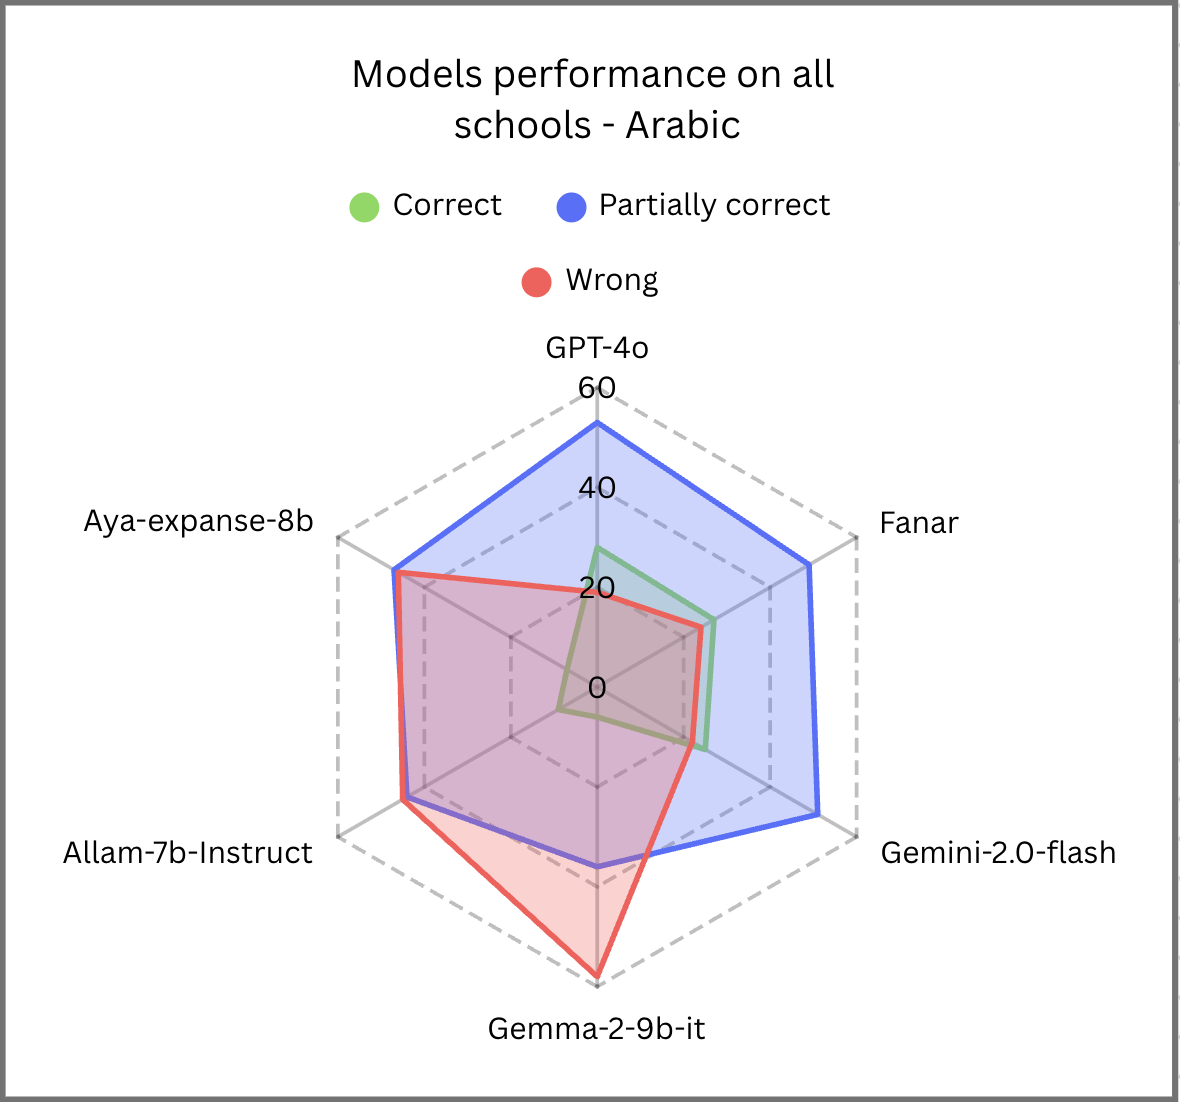
\includegraphics[width=\textwidth]{ar_all_schools.png}
        \caption{Model's performance on Arabic QA across all schools}
        \label{fig:all1}
    \end{minipage}
    \hfill
    \begin{minipage}[b]{0.48\textwidth}
        \centering
        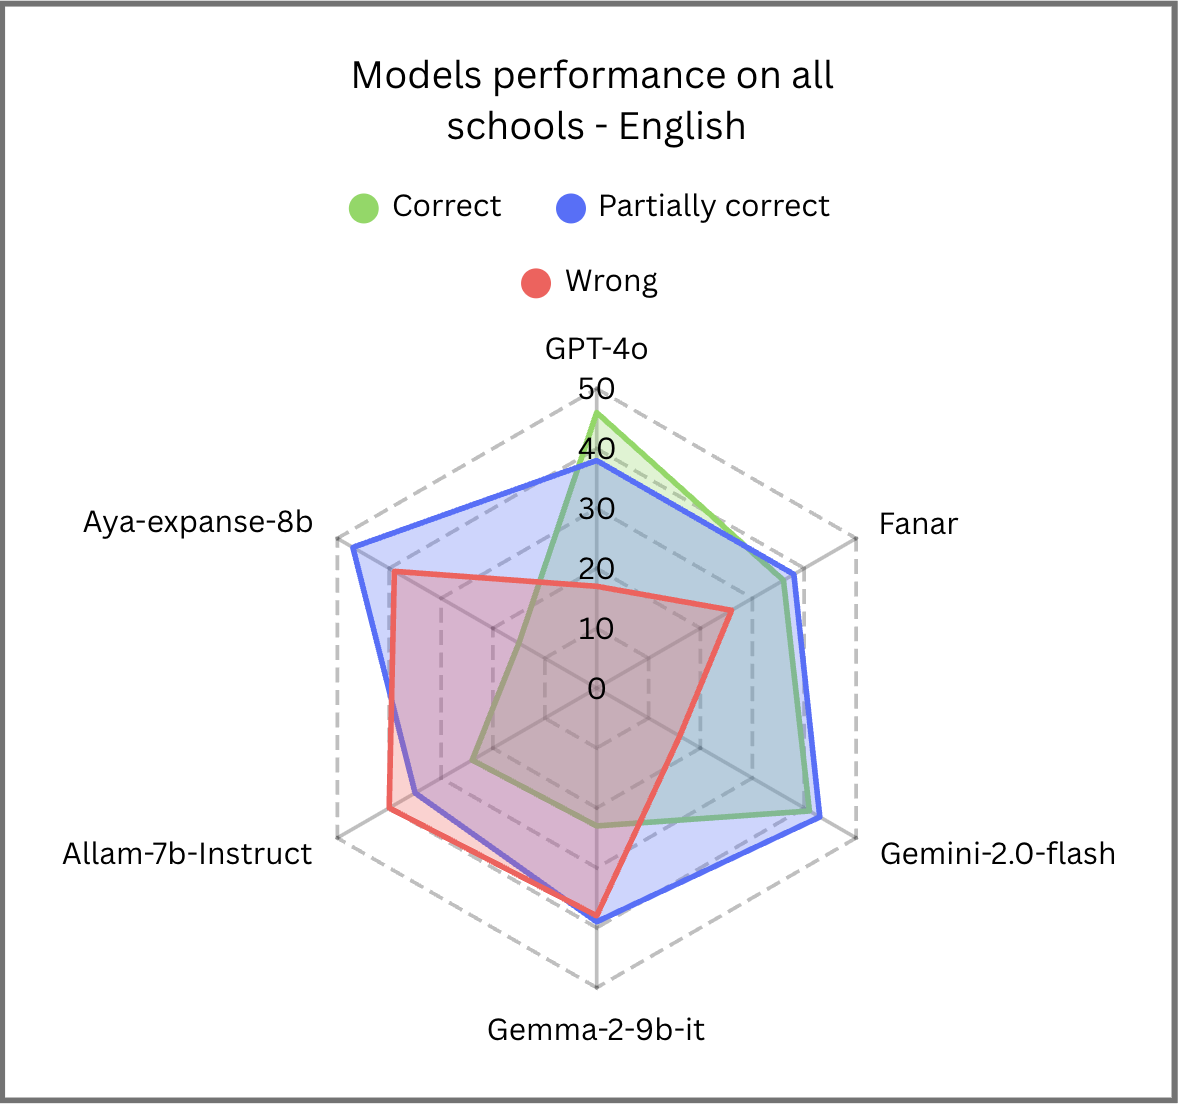
\includegraphics[width=\textwidth]{en_all_schools.png}
        \caption{Model's performance on English QA across all schools}
        \label{fig:all2}
    \end{minipage}
\end{figure}

% \textbf{Model Consistency Across Languages:} While the overall aggregated performance across languages appears relatively close, a more detailed analysis by school reveals notable differences between Arabic and English outputs within the same school. Gemini 2.0 Flash and Fanar display smaller language gaps ($\approx8–12$ percentage points difference in Score 3 rates) compared to GPT-4o ($\approx20$ points). This could imply more balanced multilingual capabilities in those architectures, though their ceiling performance remains below GPT-4o. Less capable models (Gemma-2.9B-IT, Allam, Aya-Expanse) show “wrong” (Score 1) rates over 40\% in both languages, and “partially wrong” (PW) rates nearing 25–30\%. In contrast, GPT-4o and Gemini keep combined error+partial-error rates below 40\%.

% \paragraph{School-Specific Trends:} 

\begin{figure}[h]
    \centering
    \begin{minipage}[b]{0.48\textwidth}
    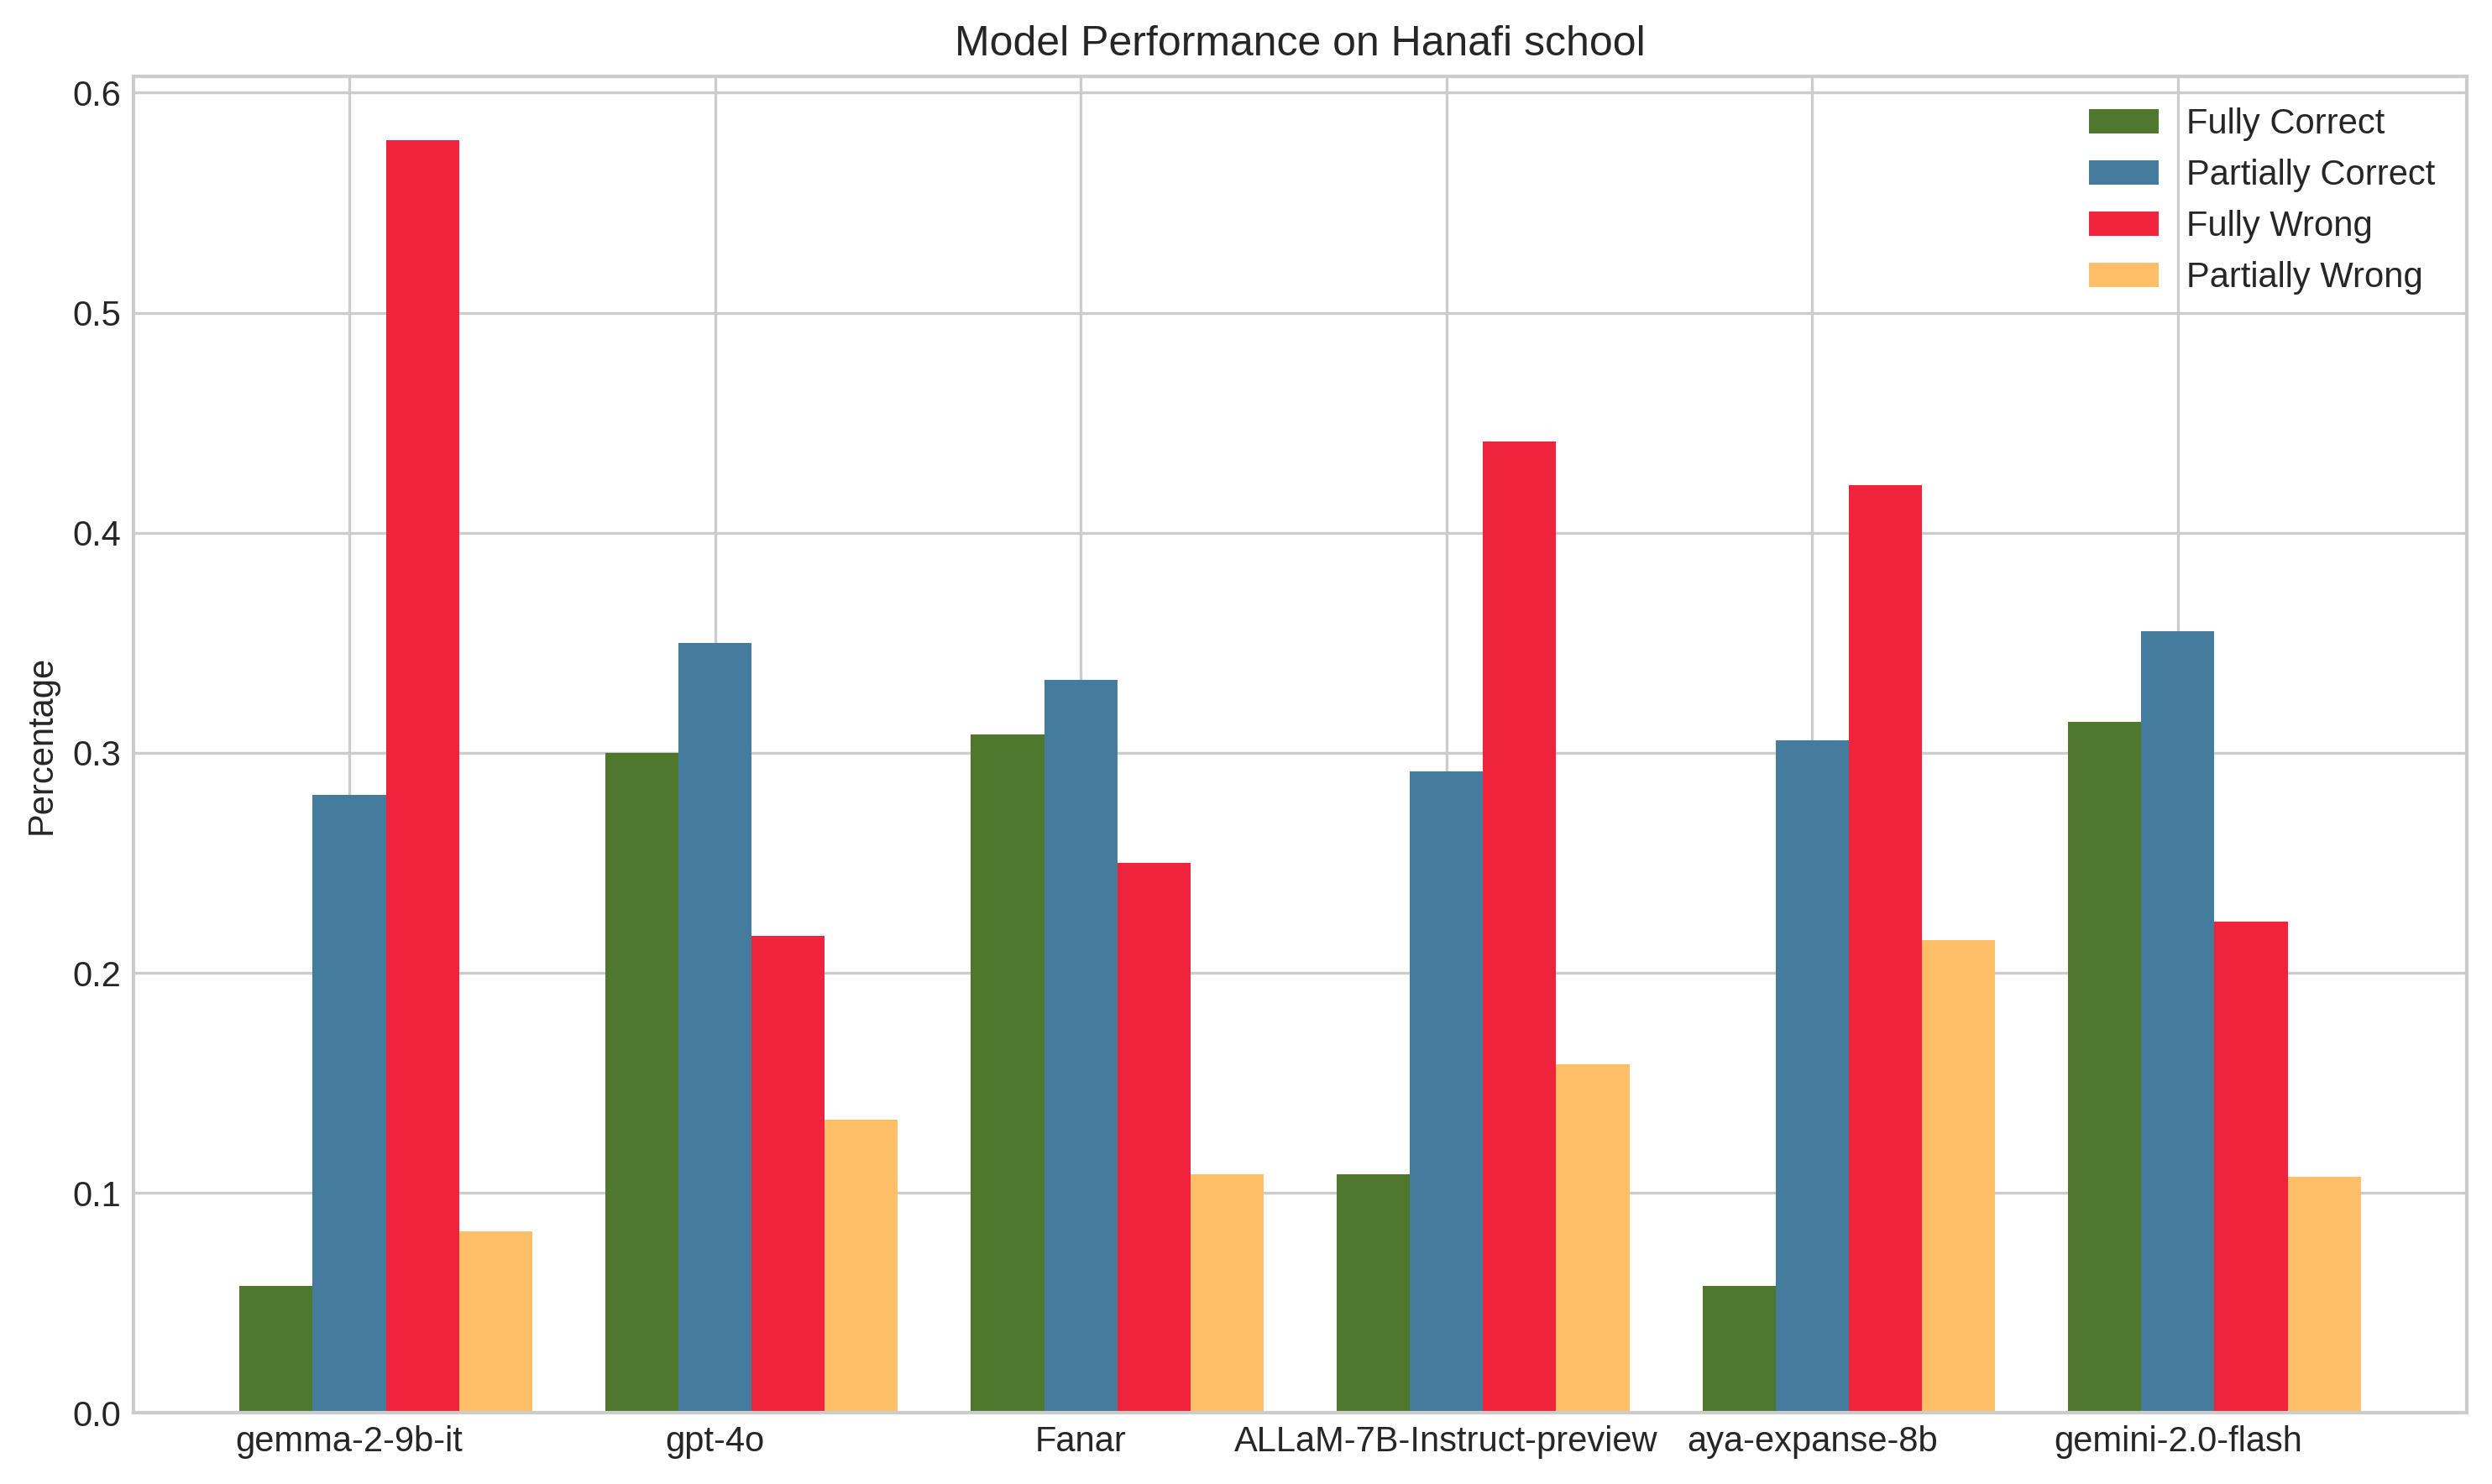
\includegraphics[height=4cm,width=0.49\linewidth]{Arabic_Hanafi.png}
    \hfill
    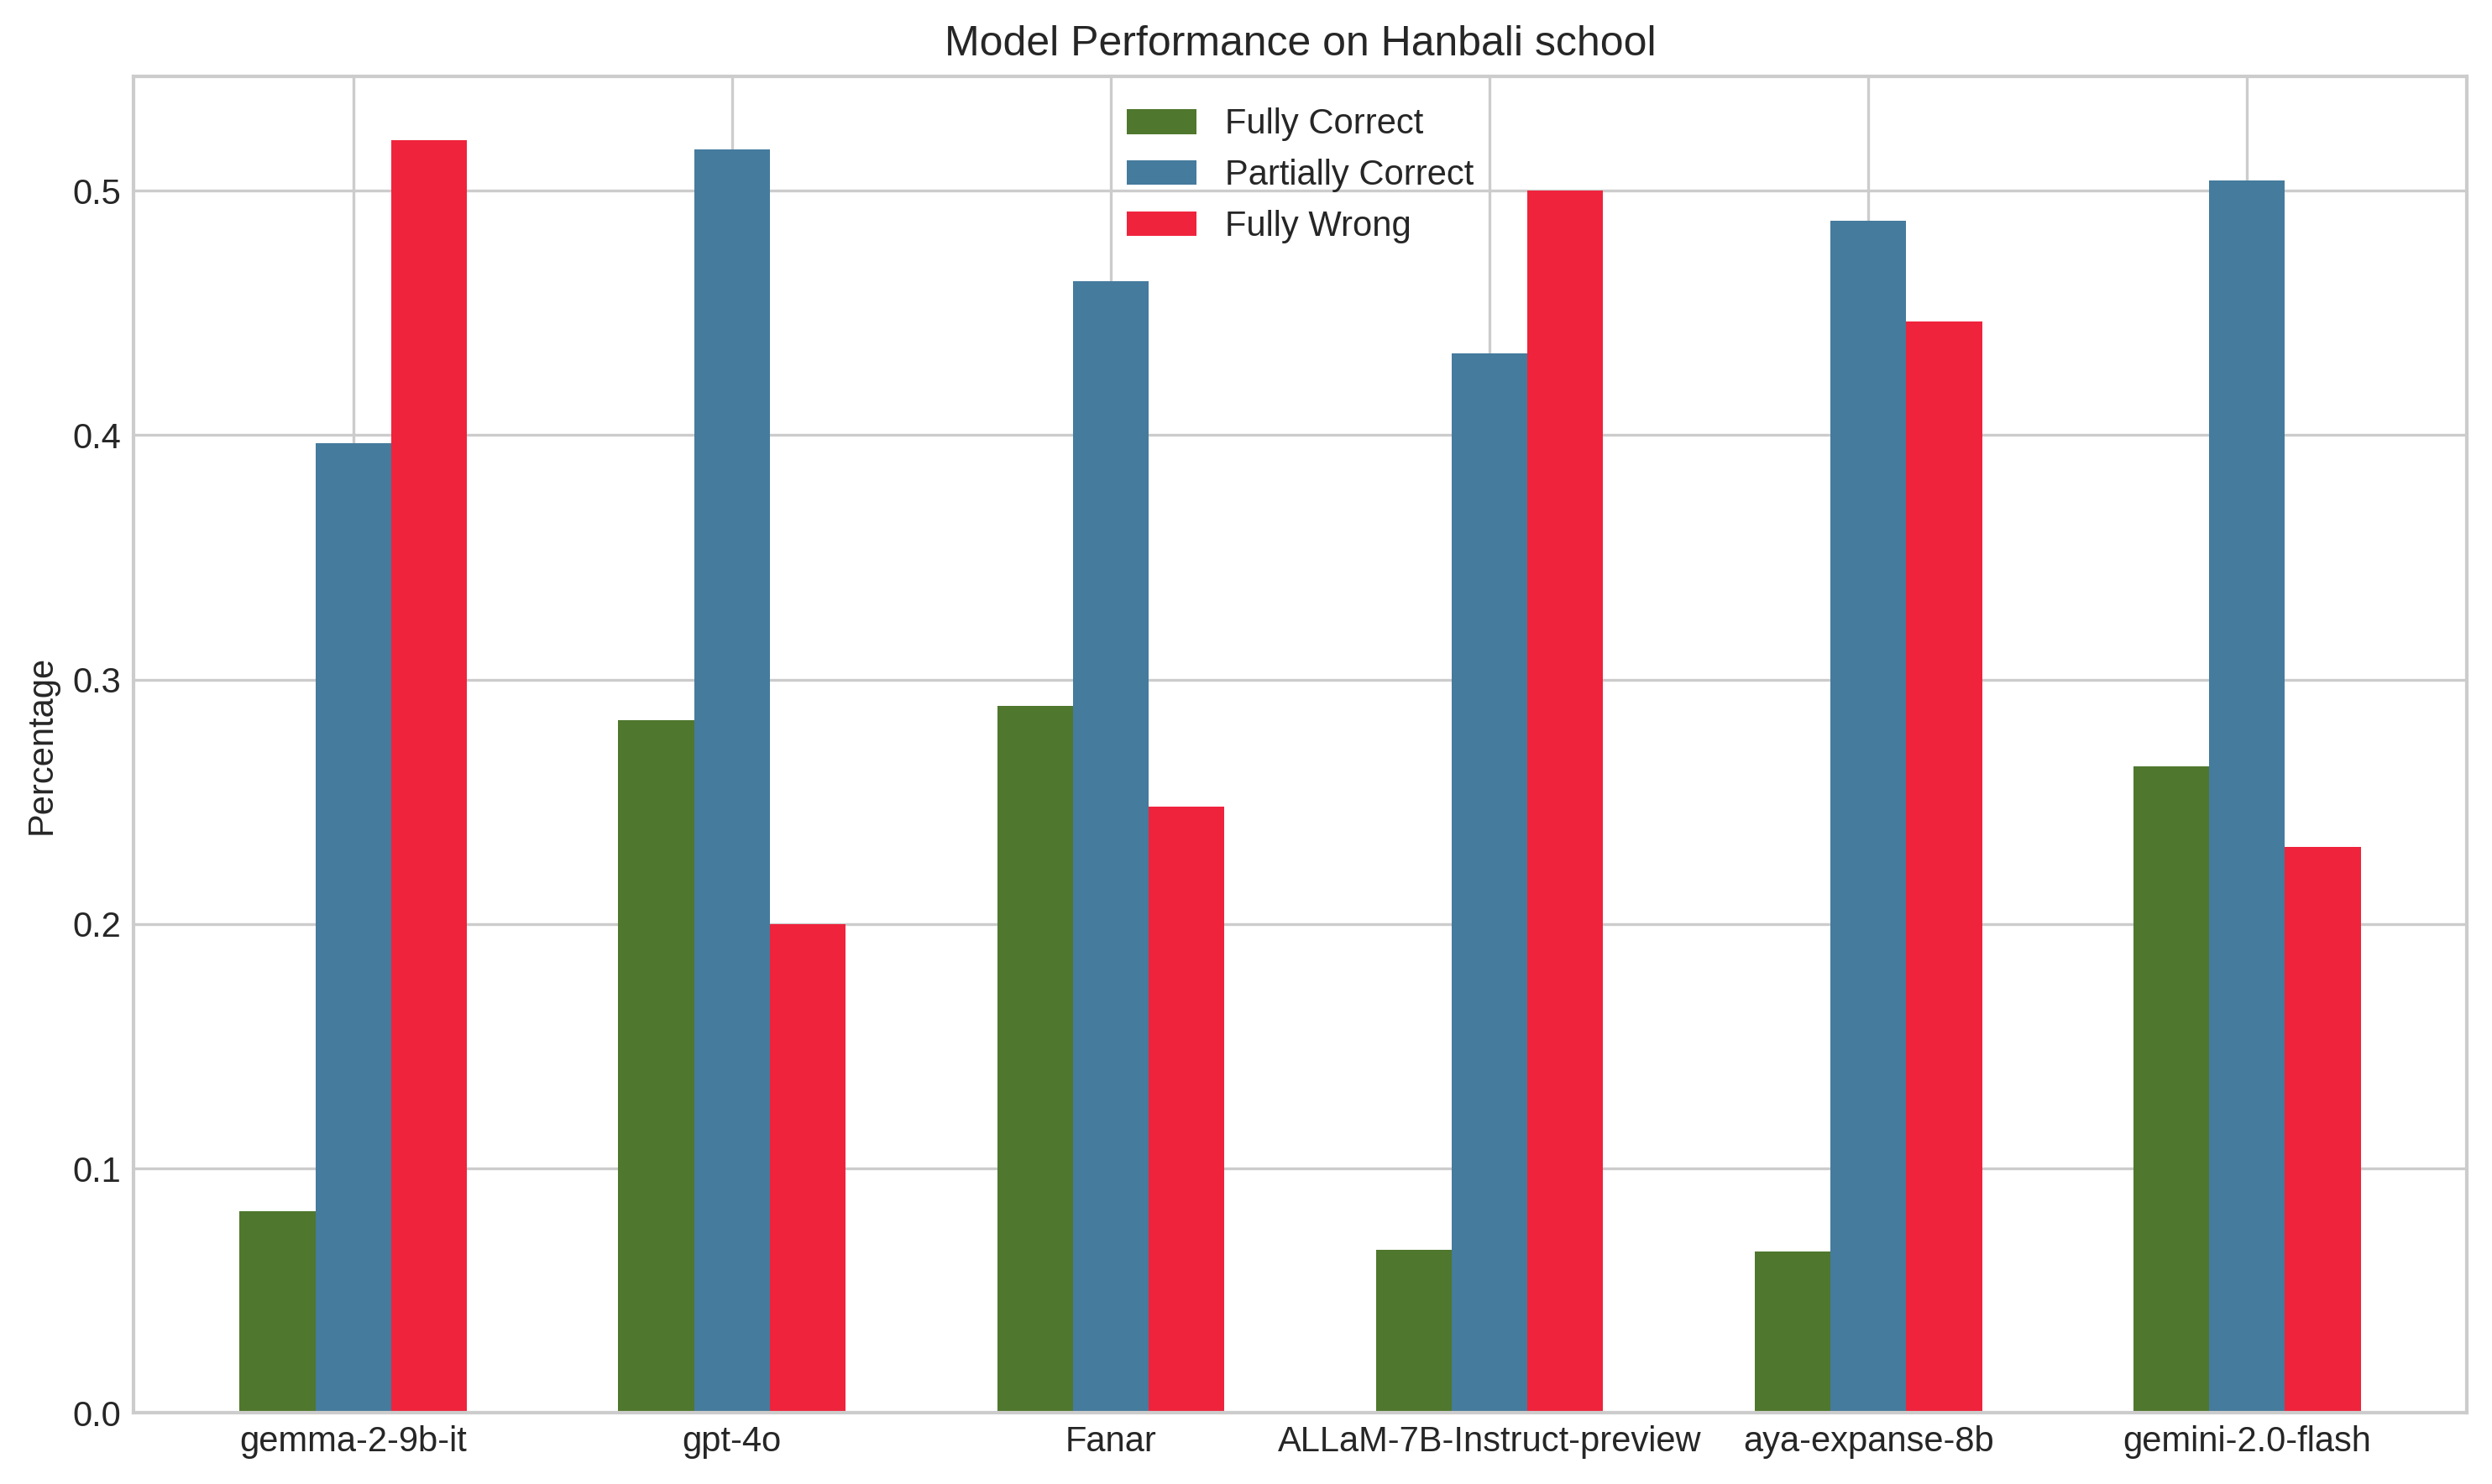
\includegraphics[height=4cm,width=0.49\linewidth]{Arabic_Hanbali.png}
    \end{minipage}
    \begin{minipage}[b]{0.48\textwidth}
    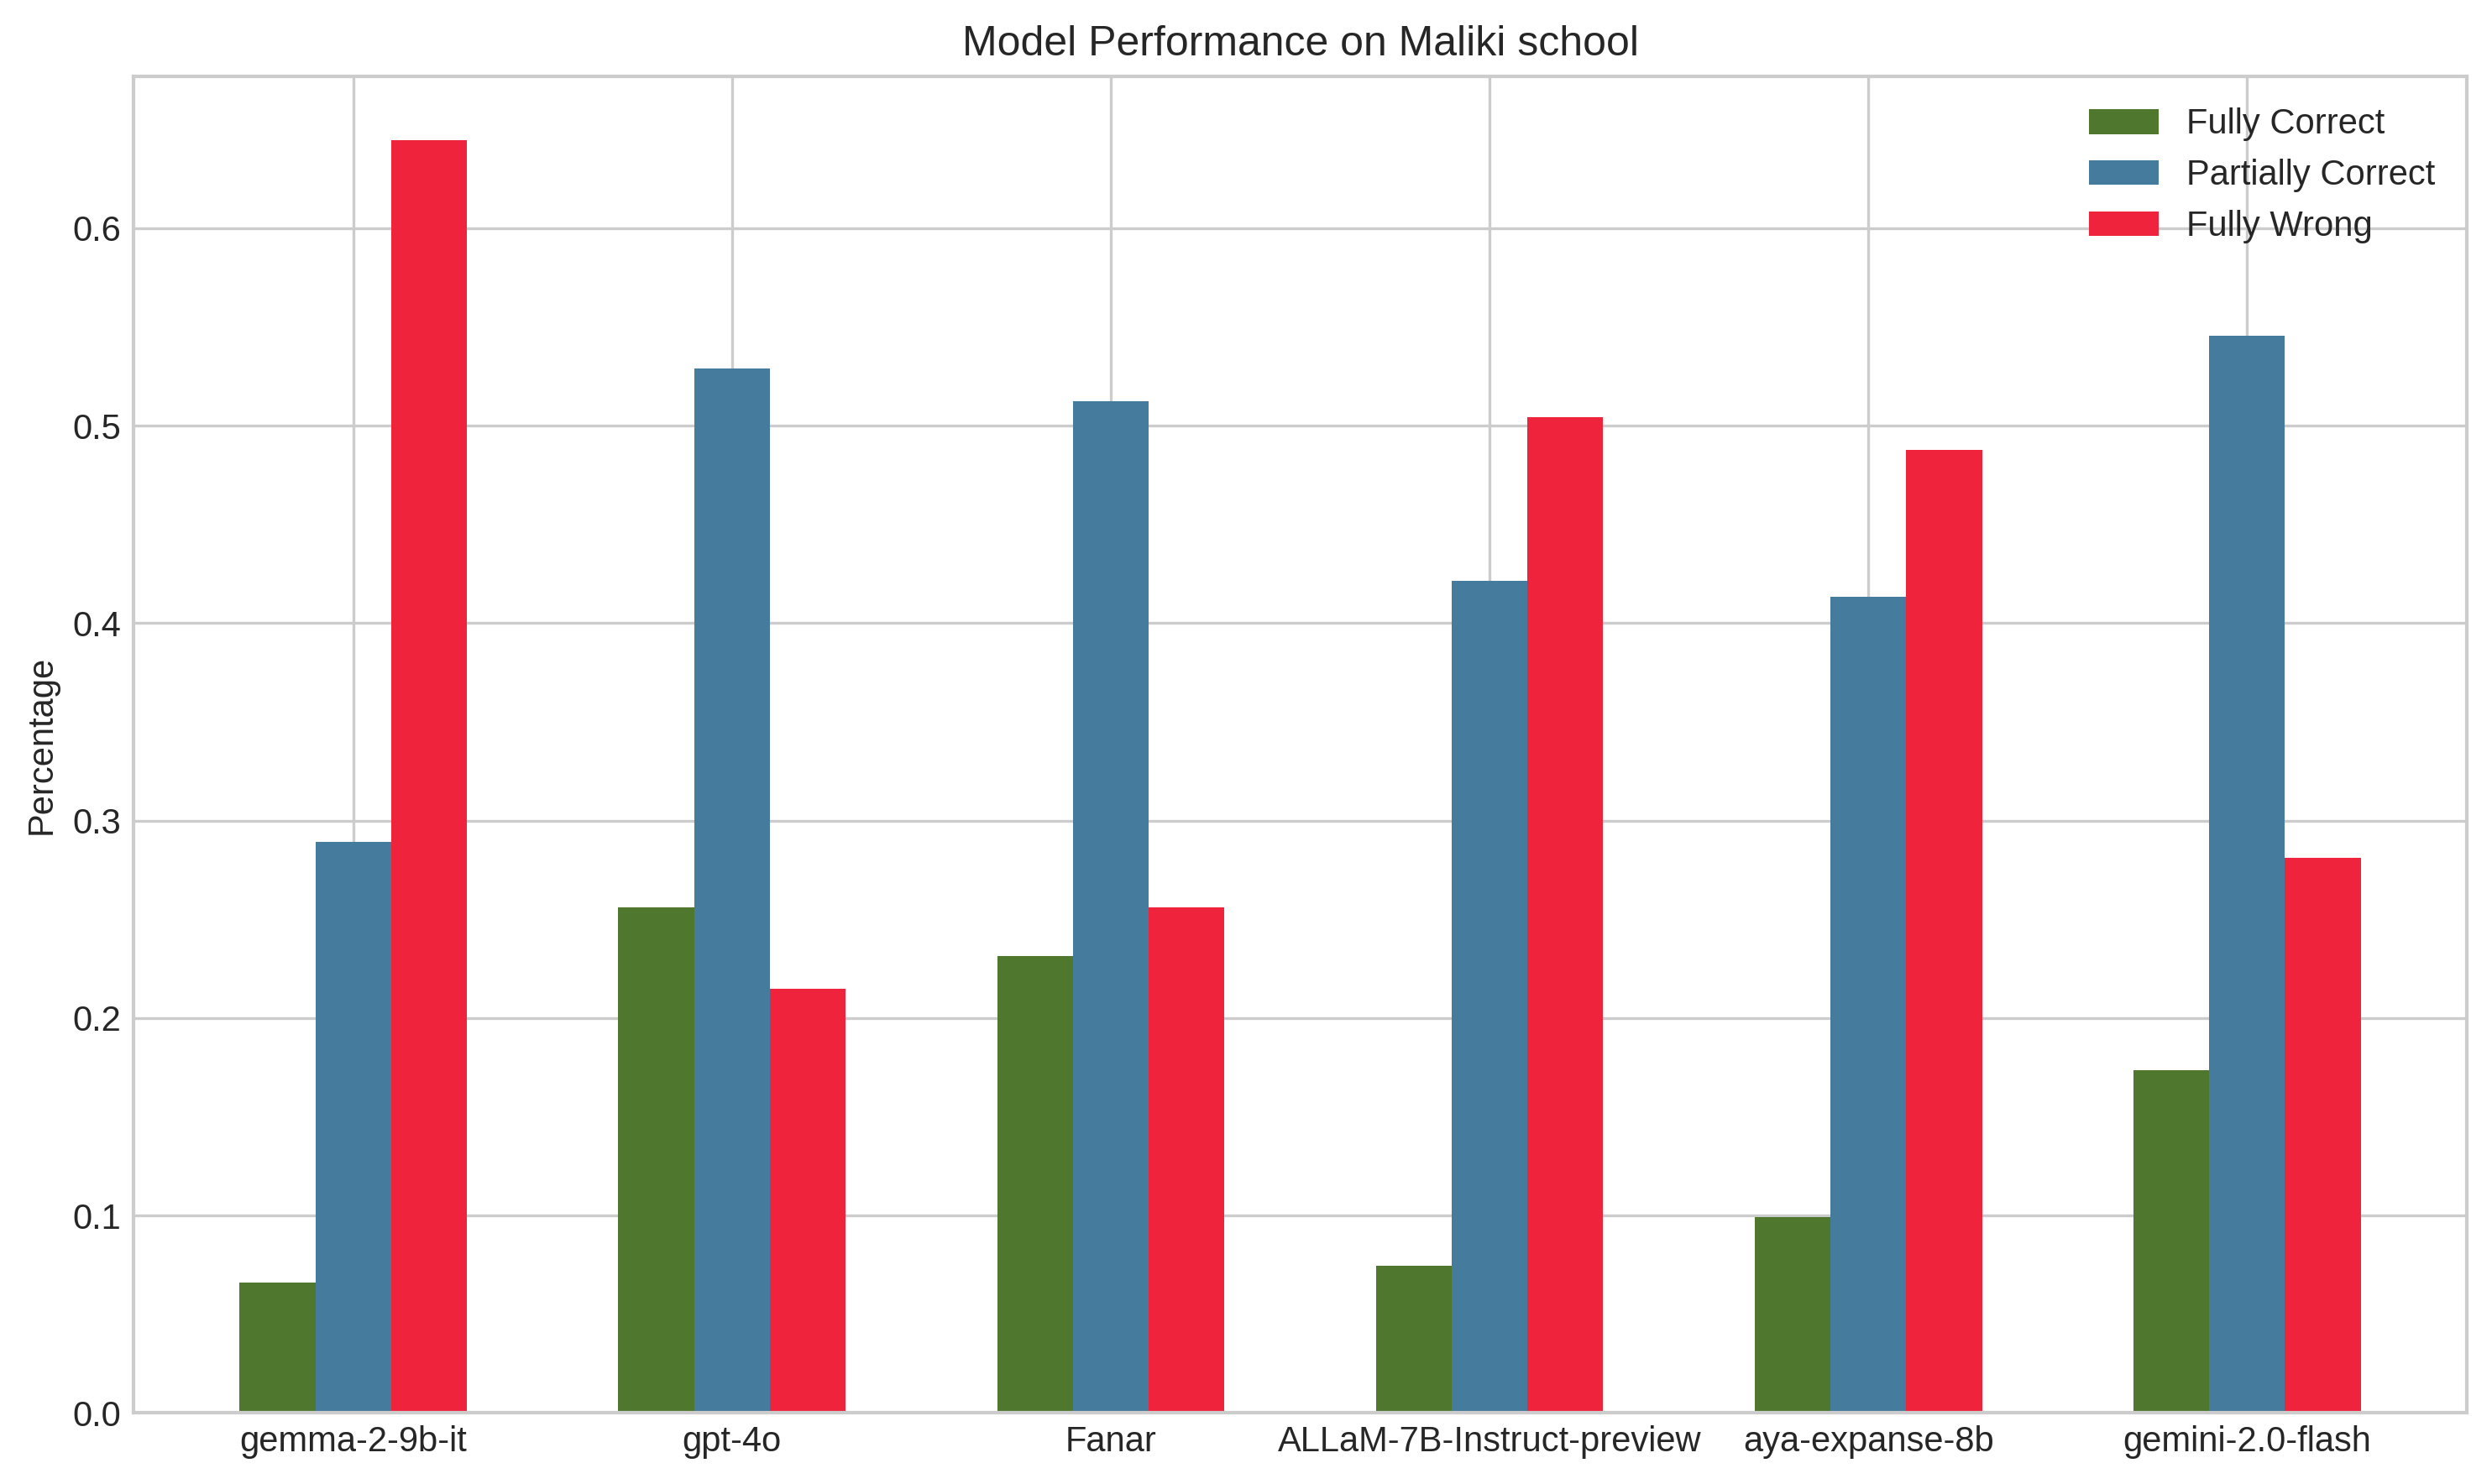
\includegraphics[height=4cm,width=0.49\linewidth]{Arabic_Maliki.png}
    \hfill
    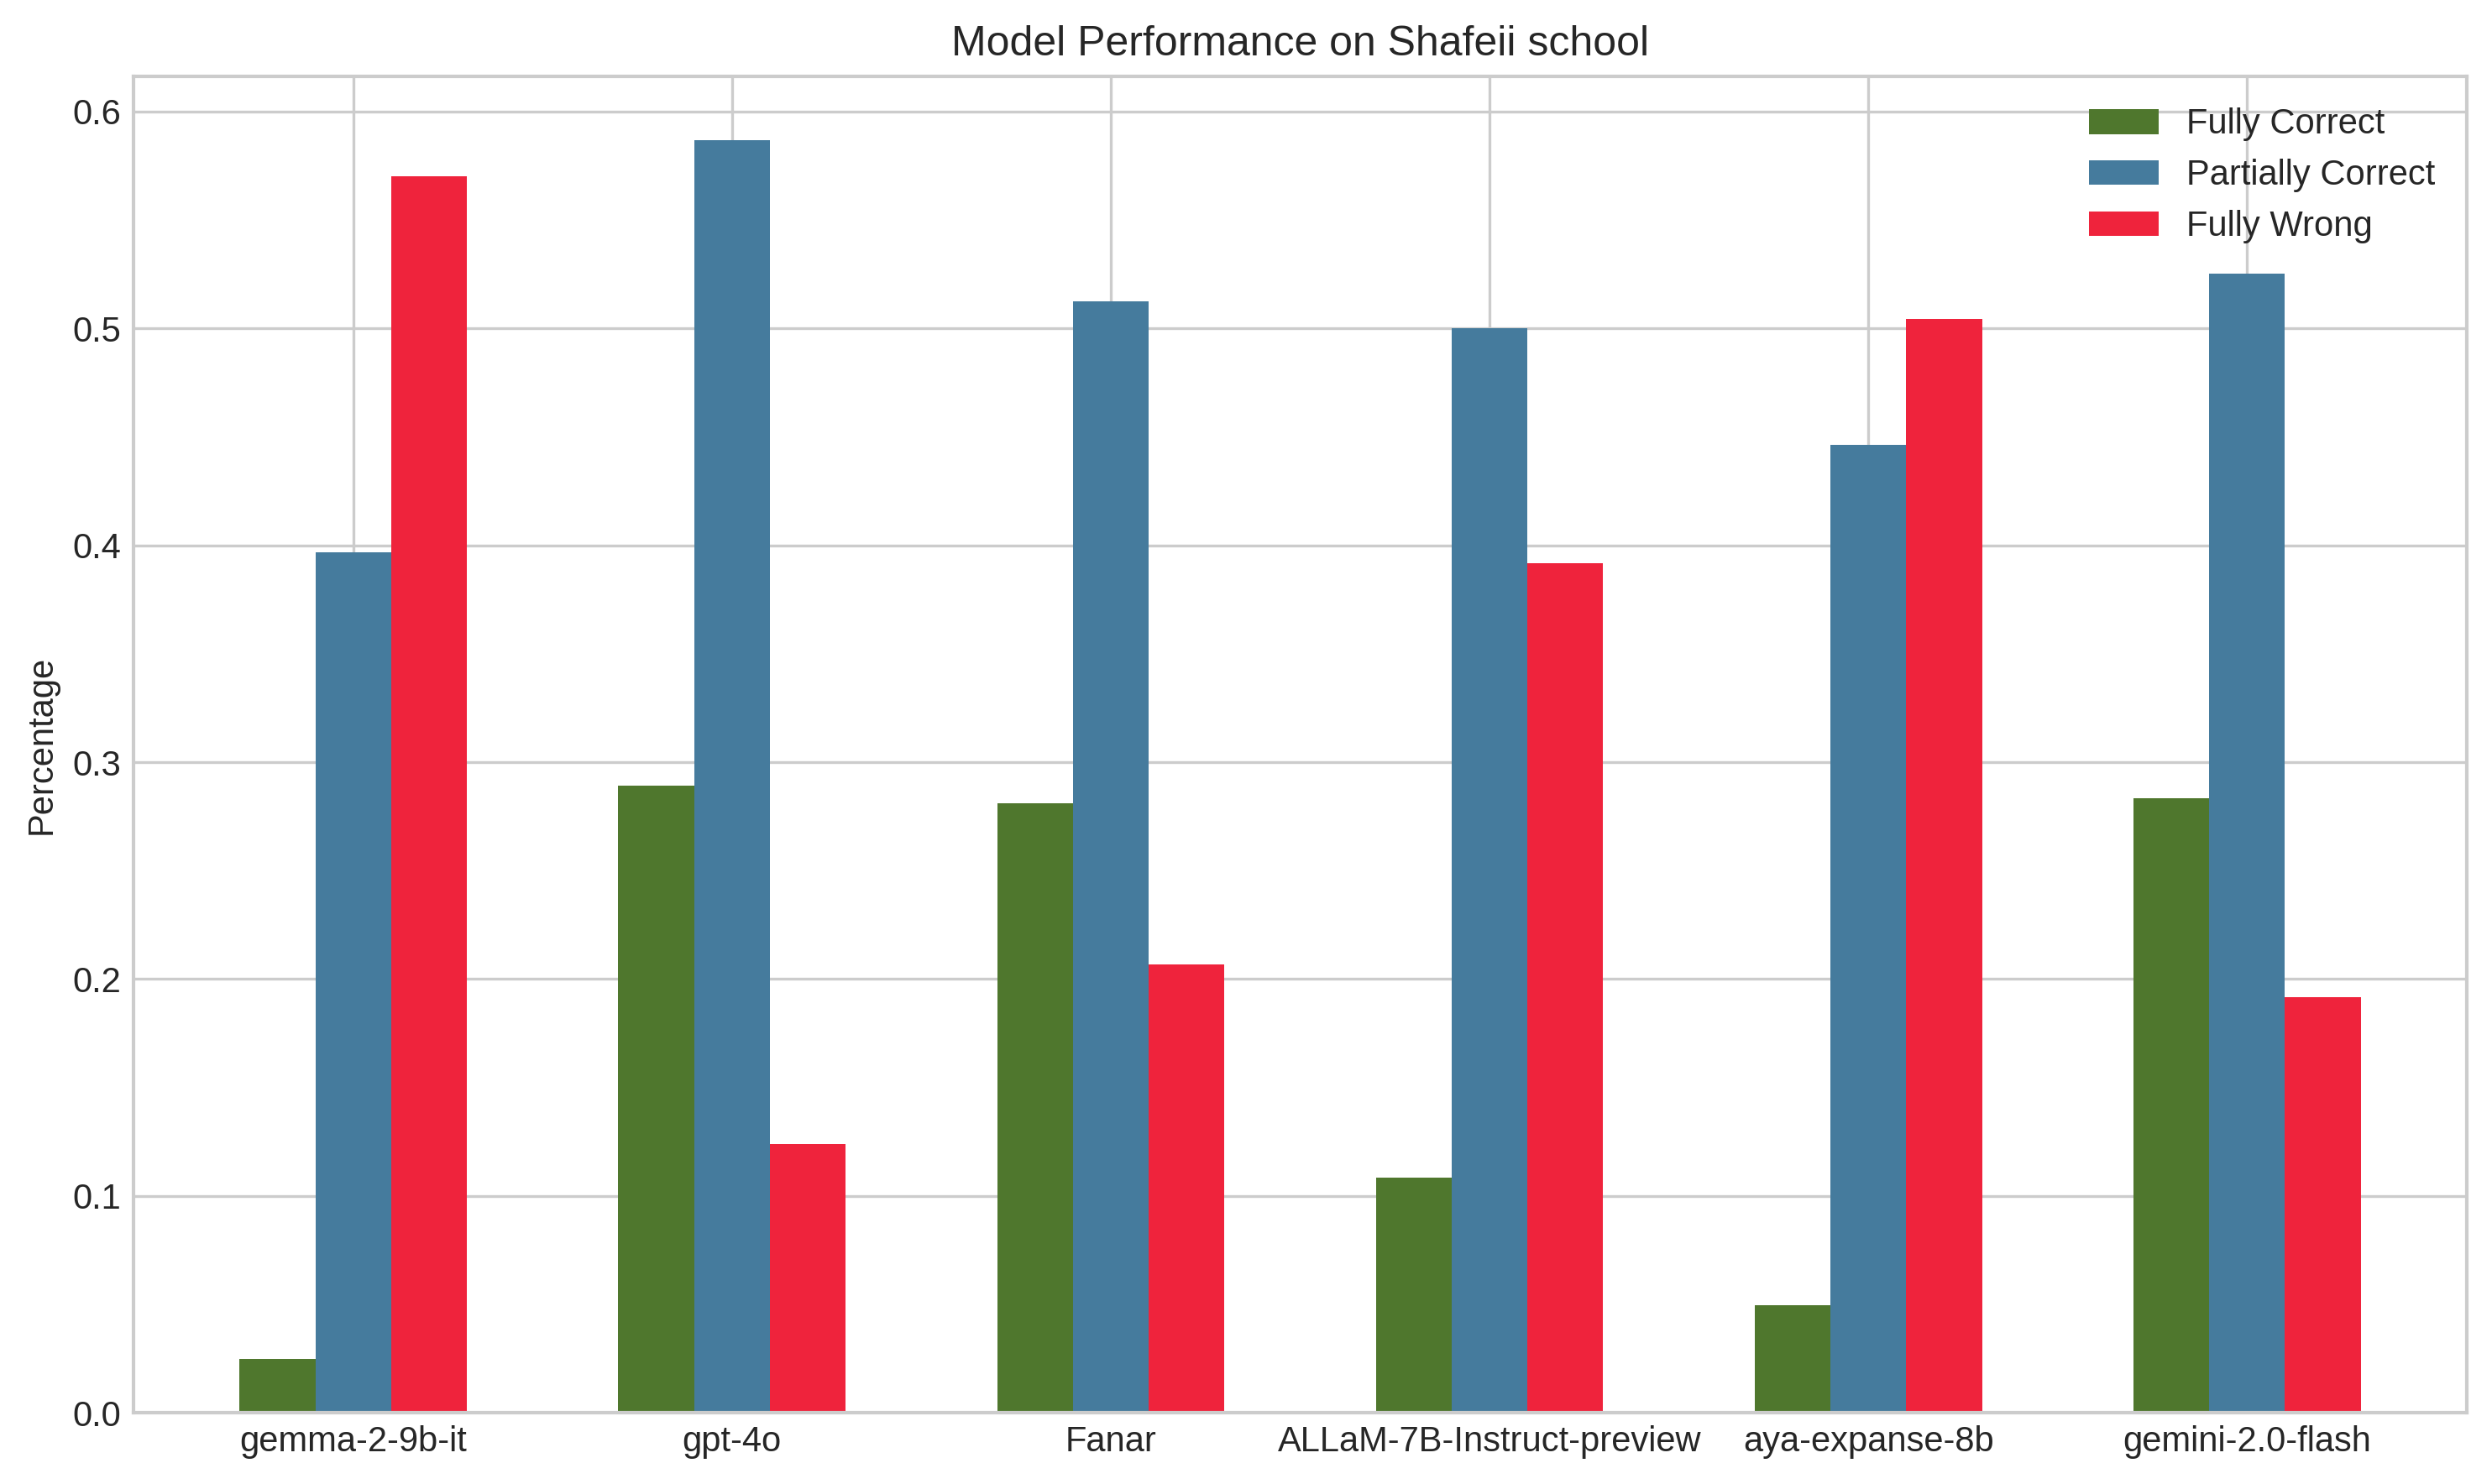
\includegraphics[height=4cm,width=0.49\linewidth]{Arabic_Shafeii.png}
    \end{minipage}
    \caption{Model's performance on Hanafi, Hanbali, Maliki, and Shafeii schools respectively on Arabic.}
    \label{fig:arabic4}
\end{figure}

\begin{figure}[h]
    \centering
    \begin{minipage}[b]{0.48\textwidth}
    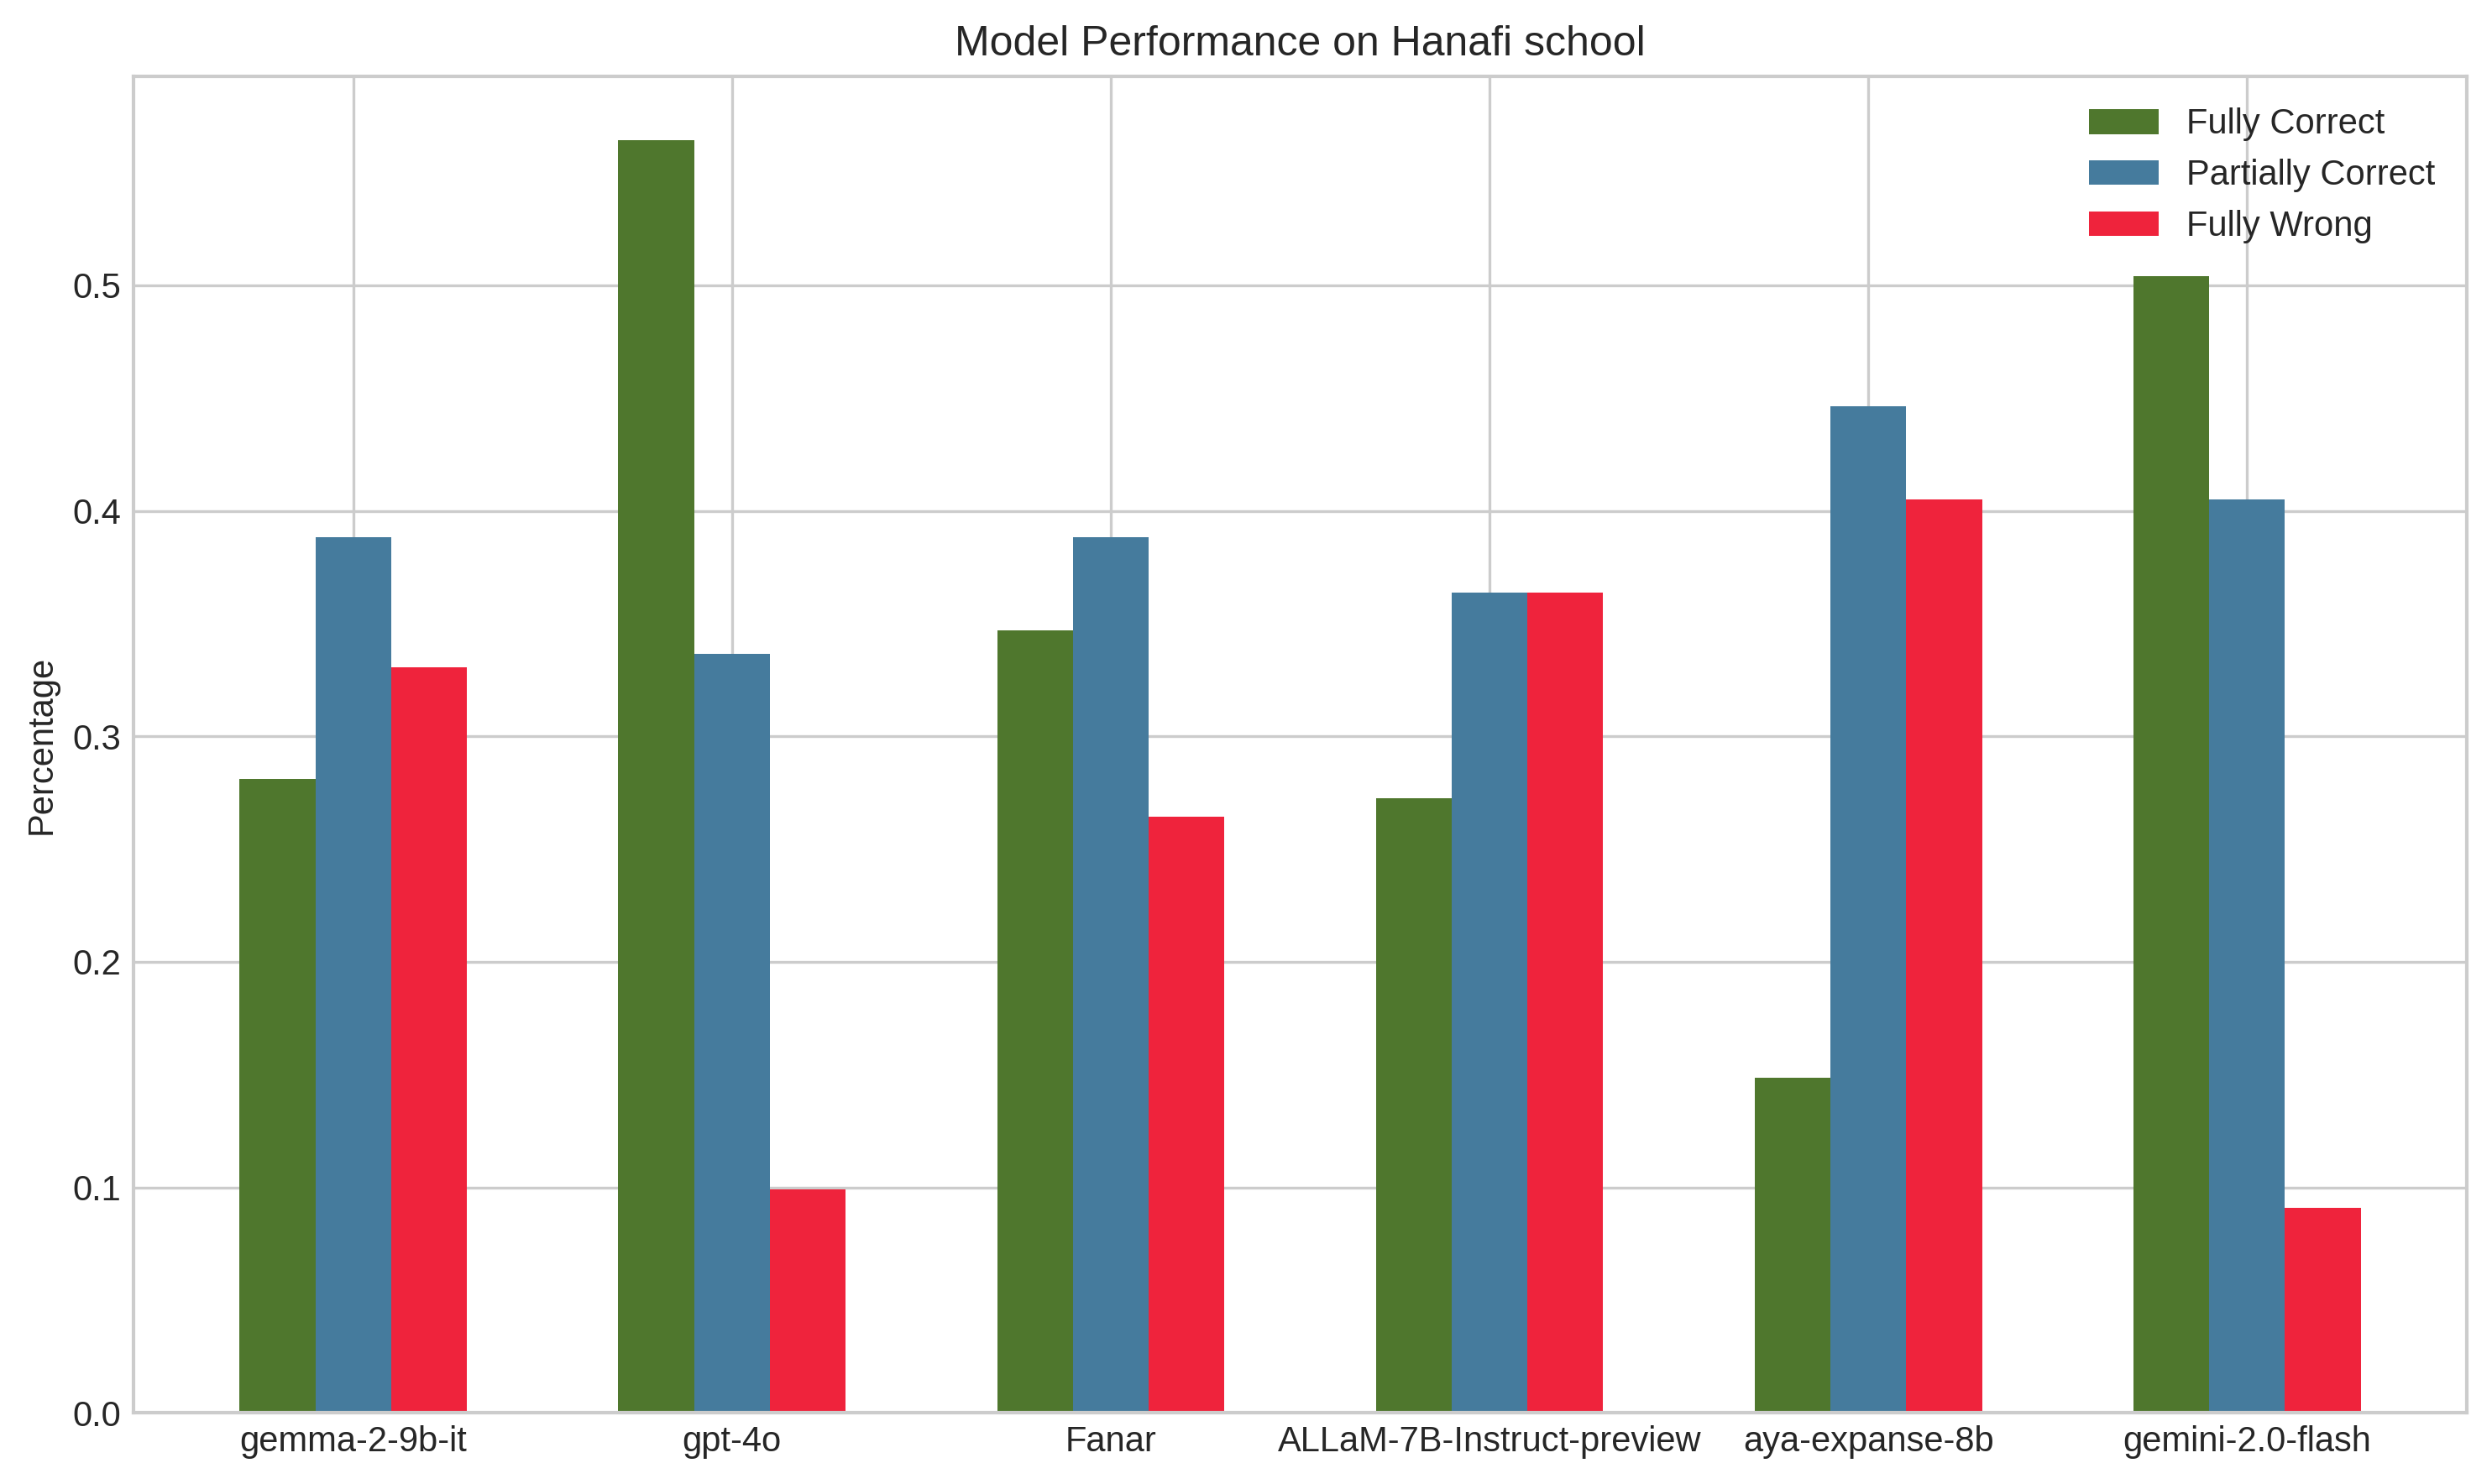
\includegraphics[height=4cm,width=0.49\linewidth]{English_Hanafi.png}
    \hfill
    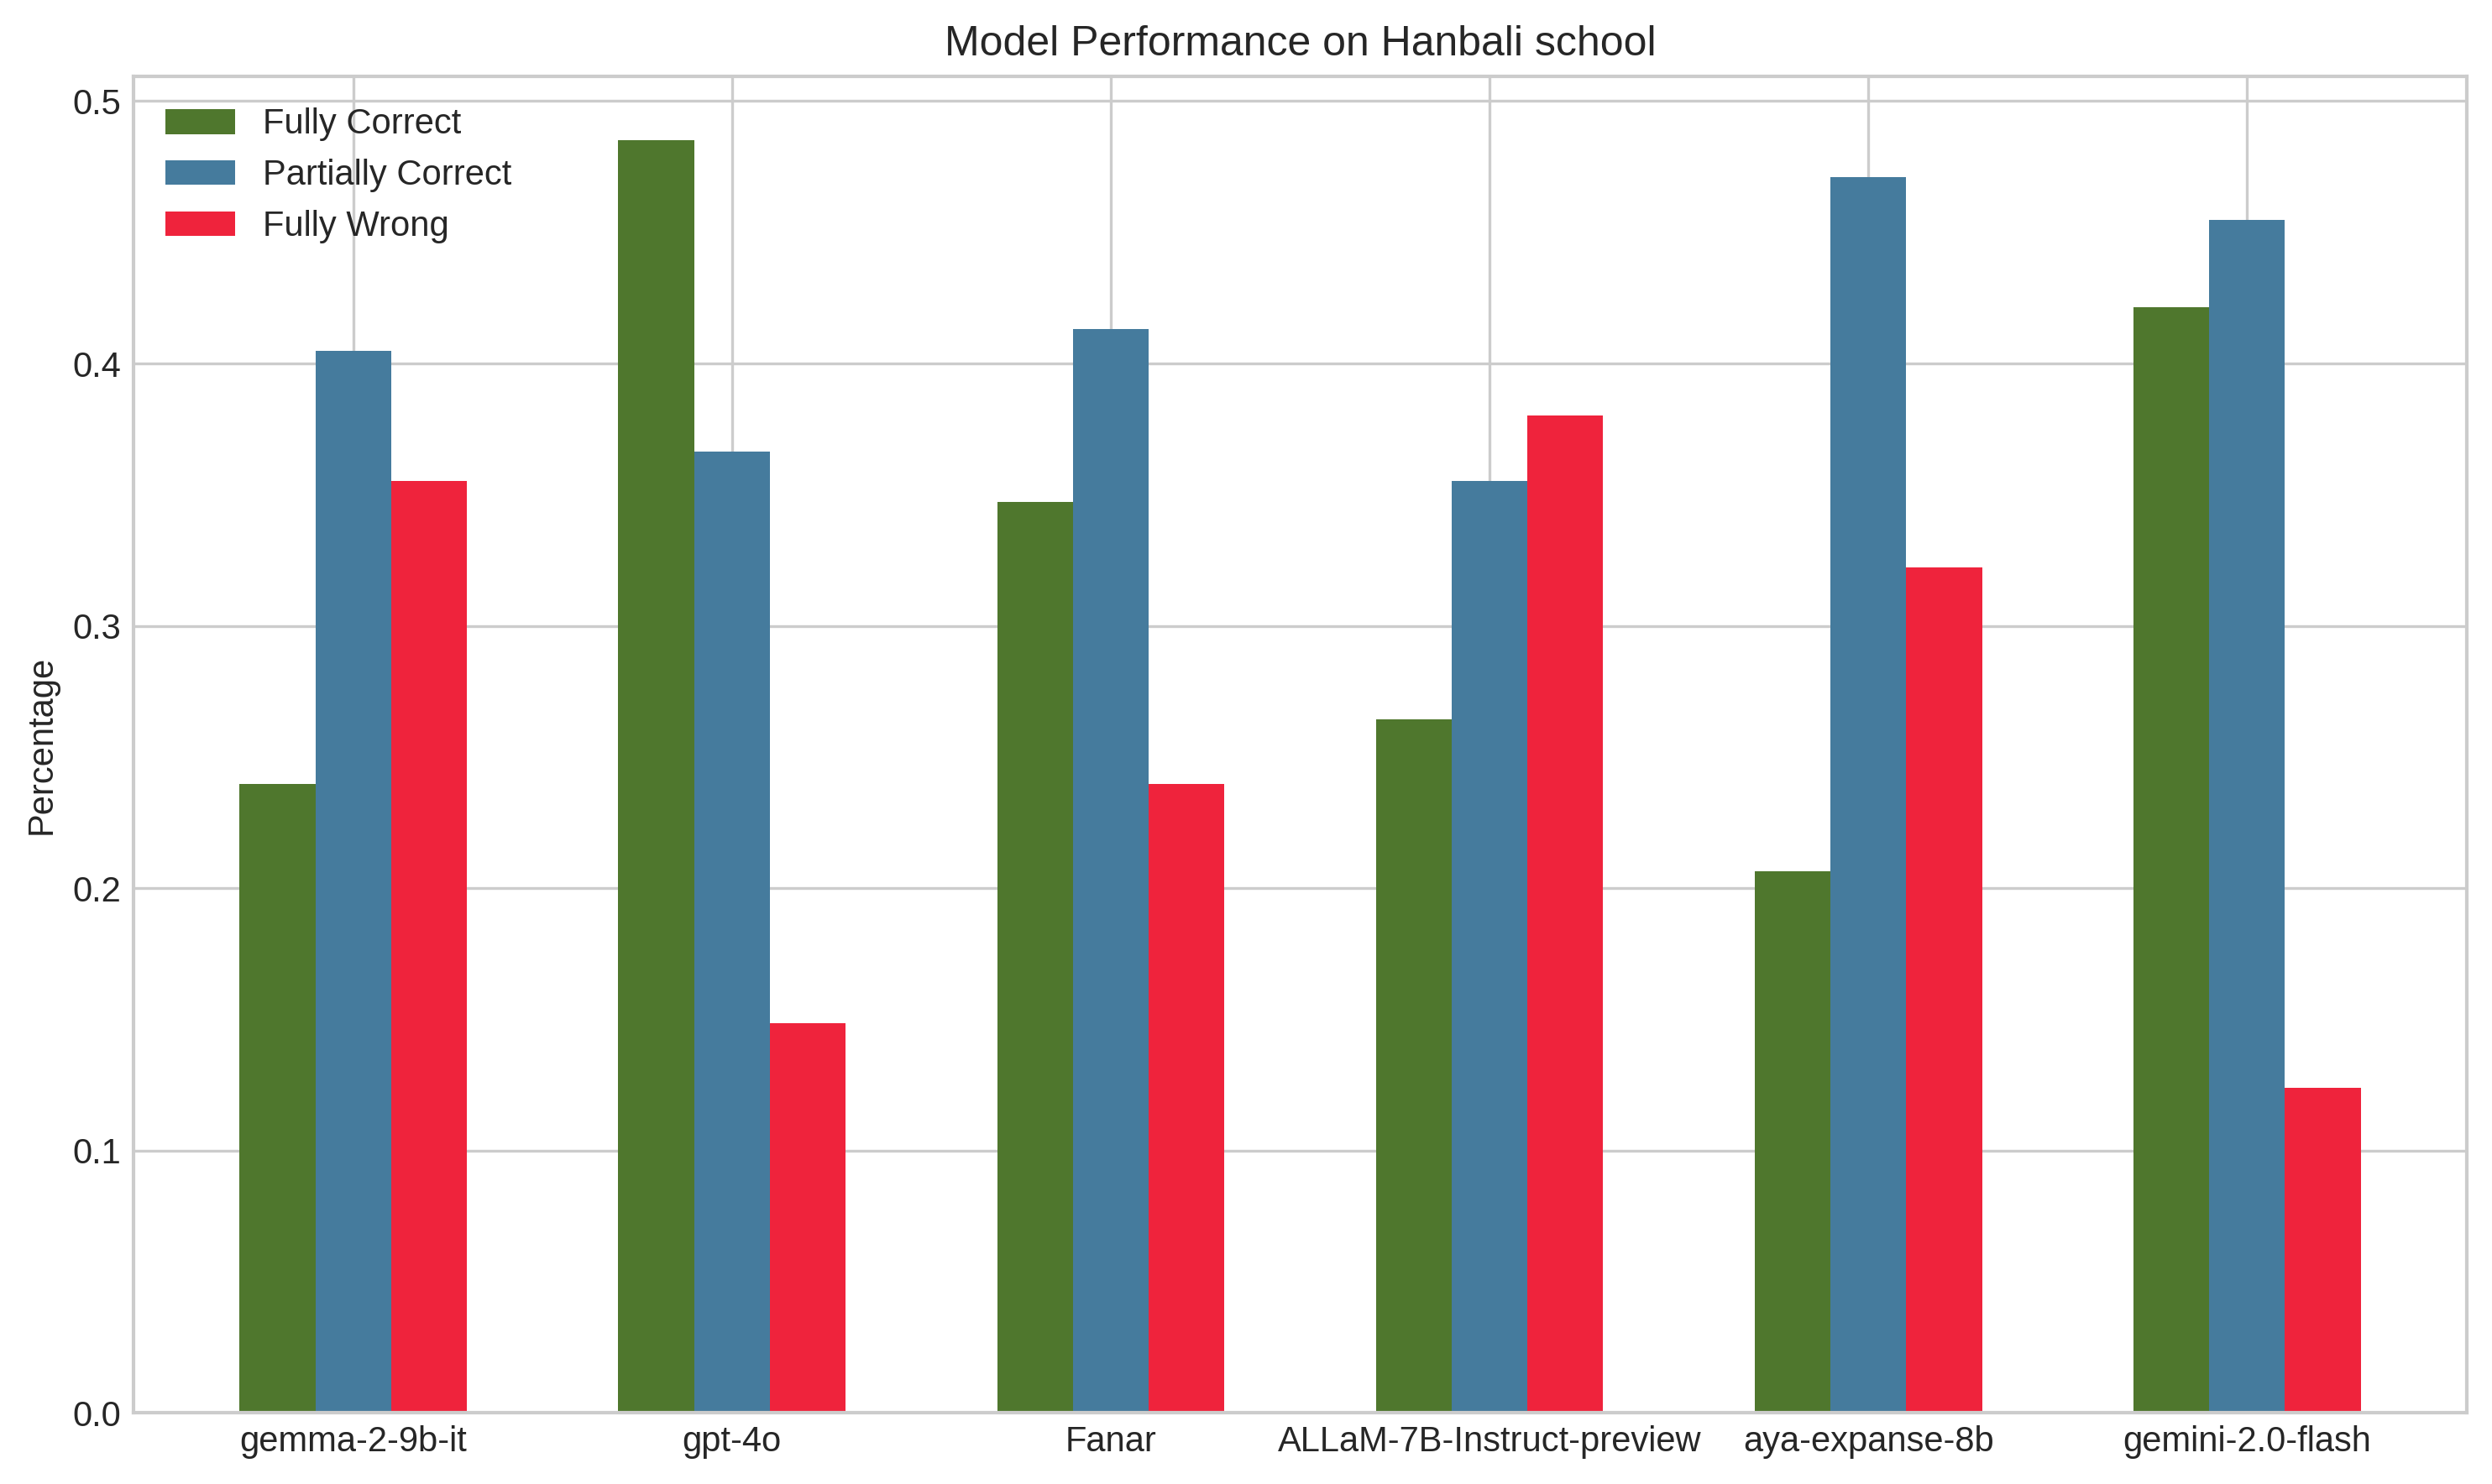
\includegraphics[height=4cm,width=0.49\linewidth]{English_Hanbali.png}
    \end{minipage}
    \begin{minipage}[b]{0.48\textwidth}
    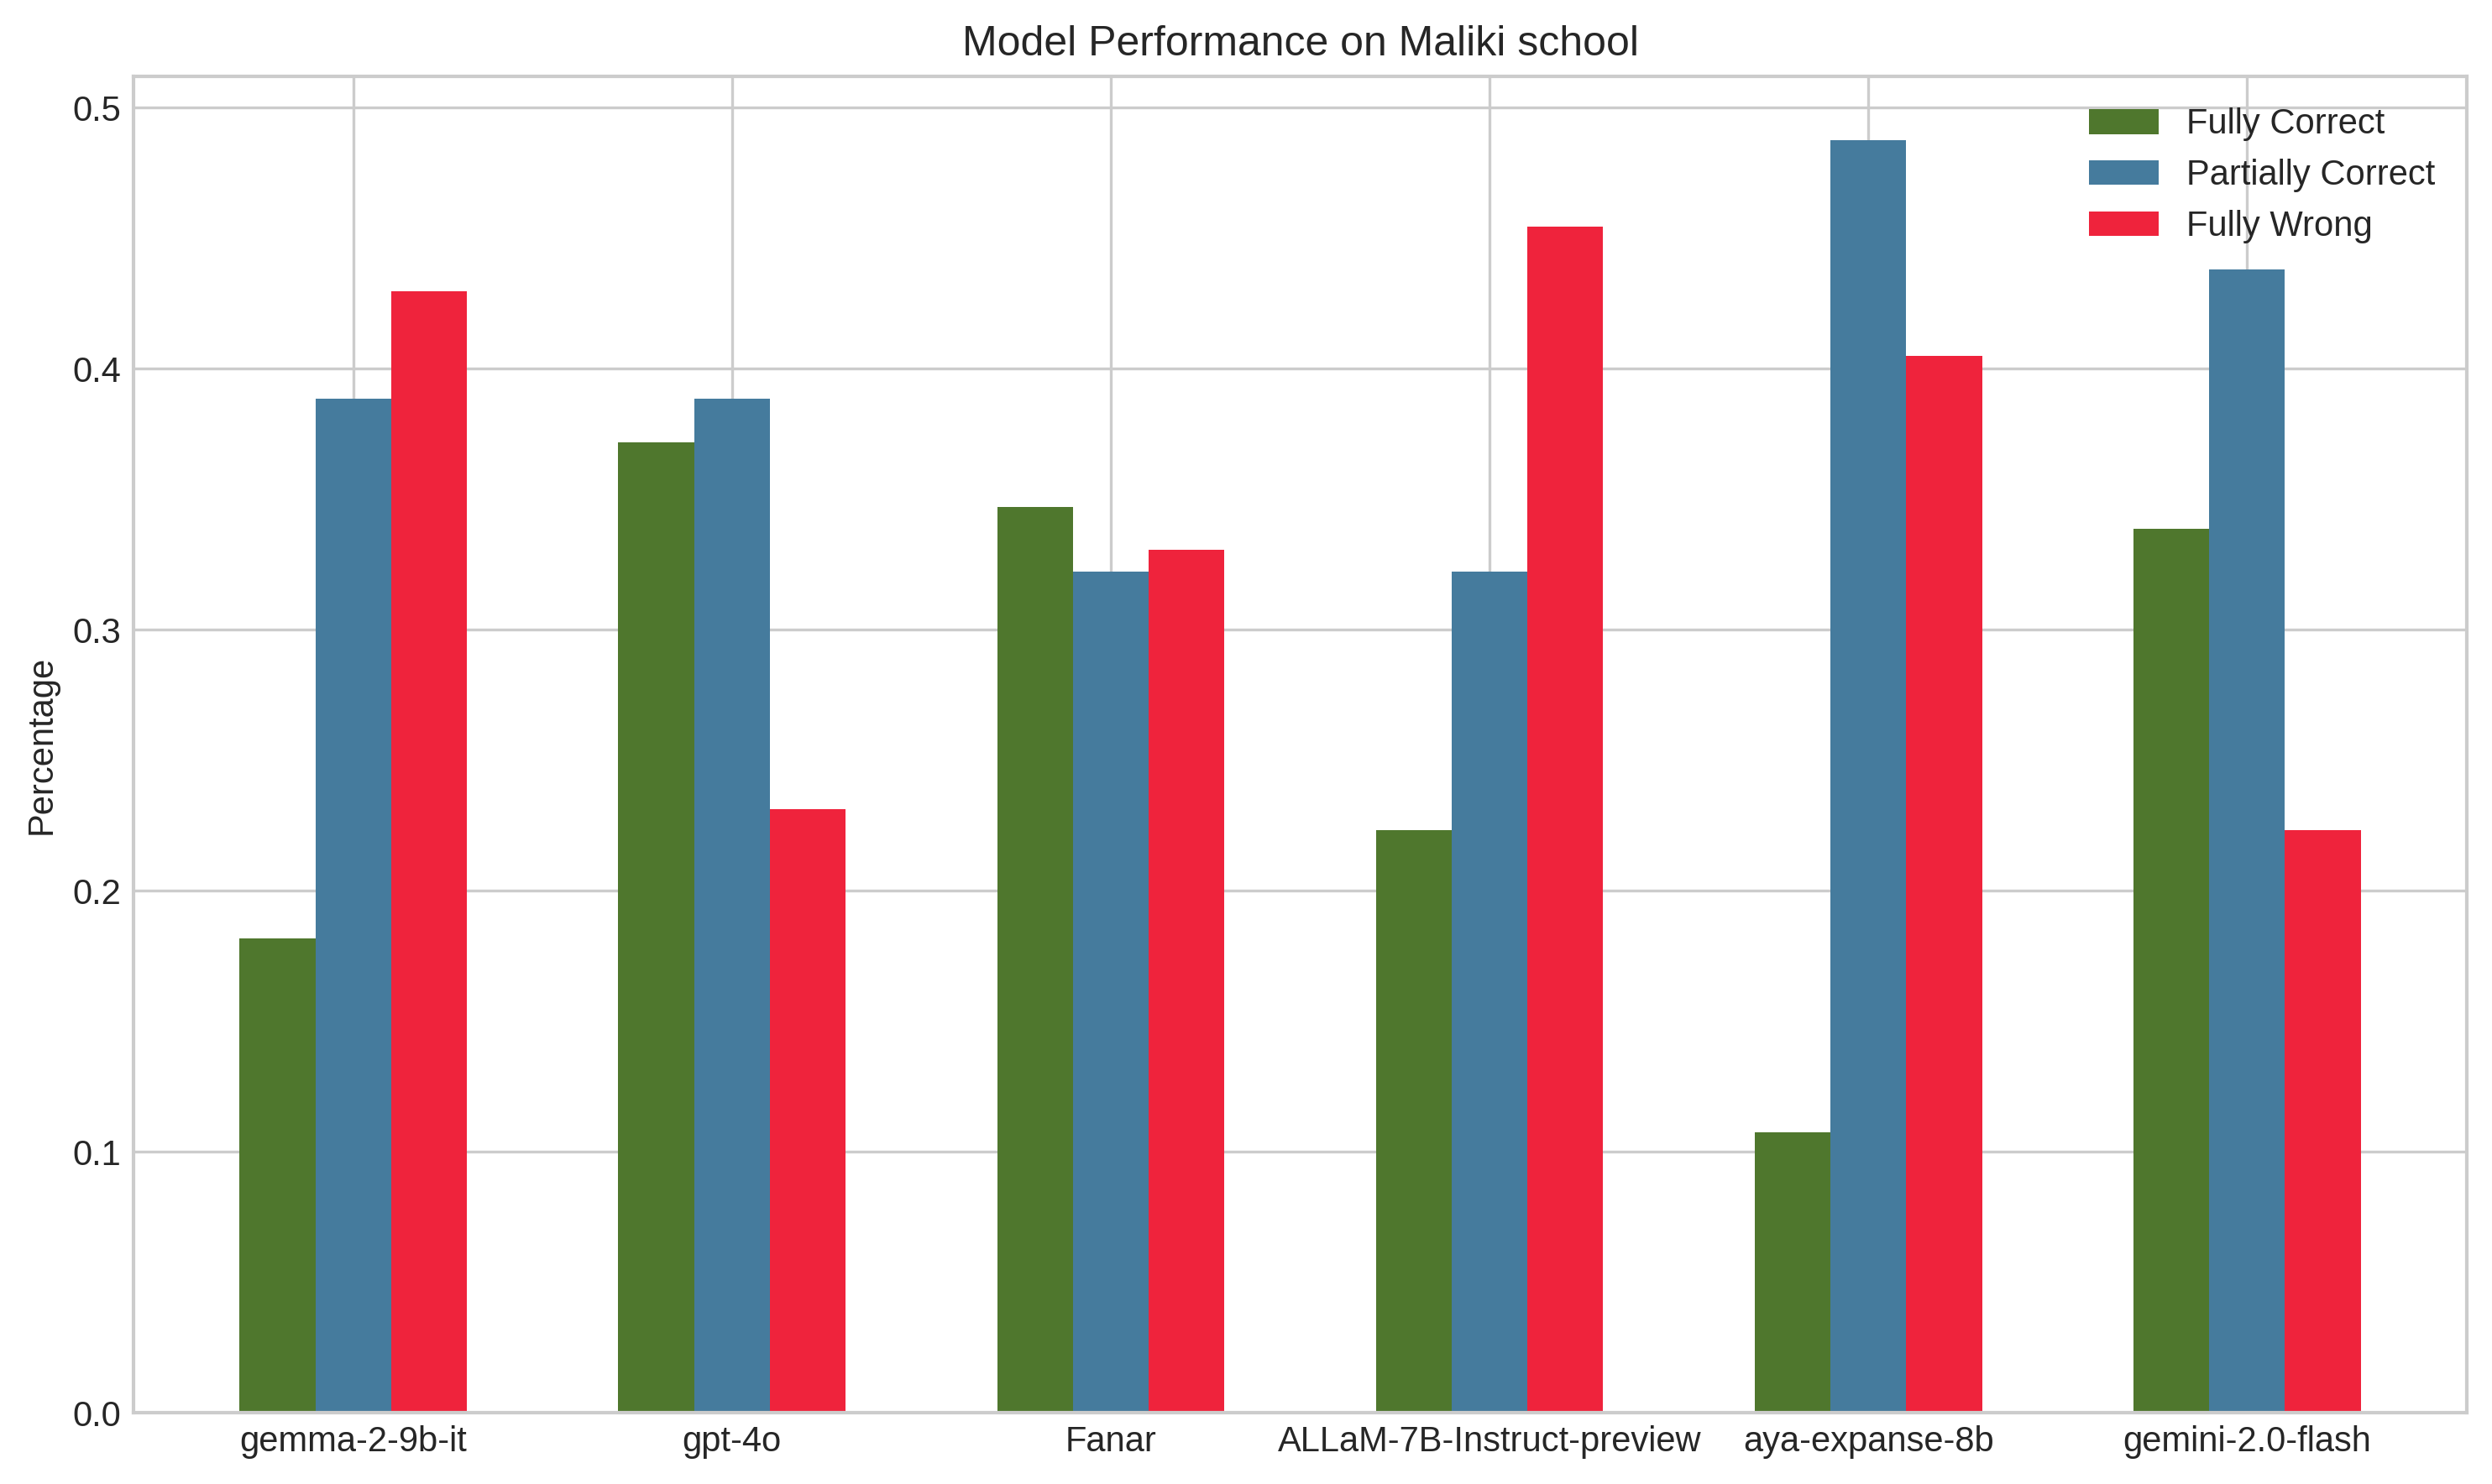
\includegraphics[height=4cm,width=0.49\linewidth]{English_Maliki.png}
    \hfill
    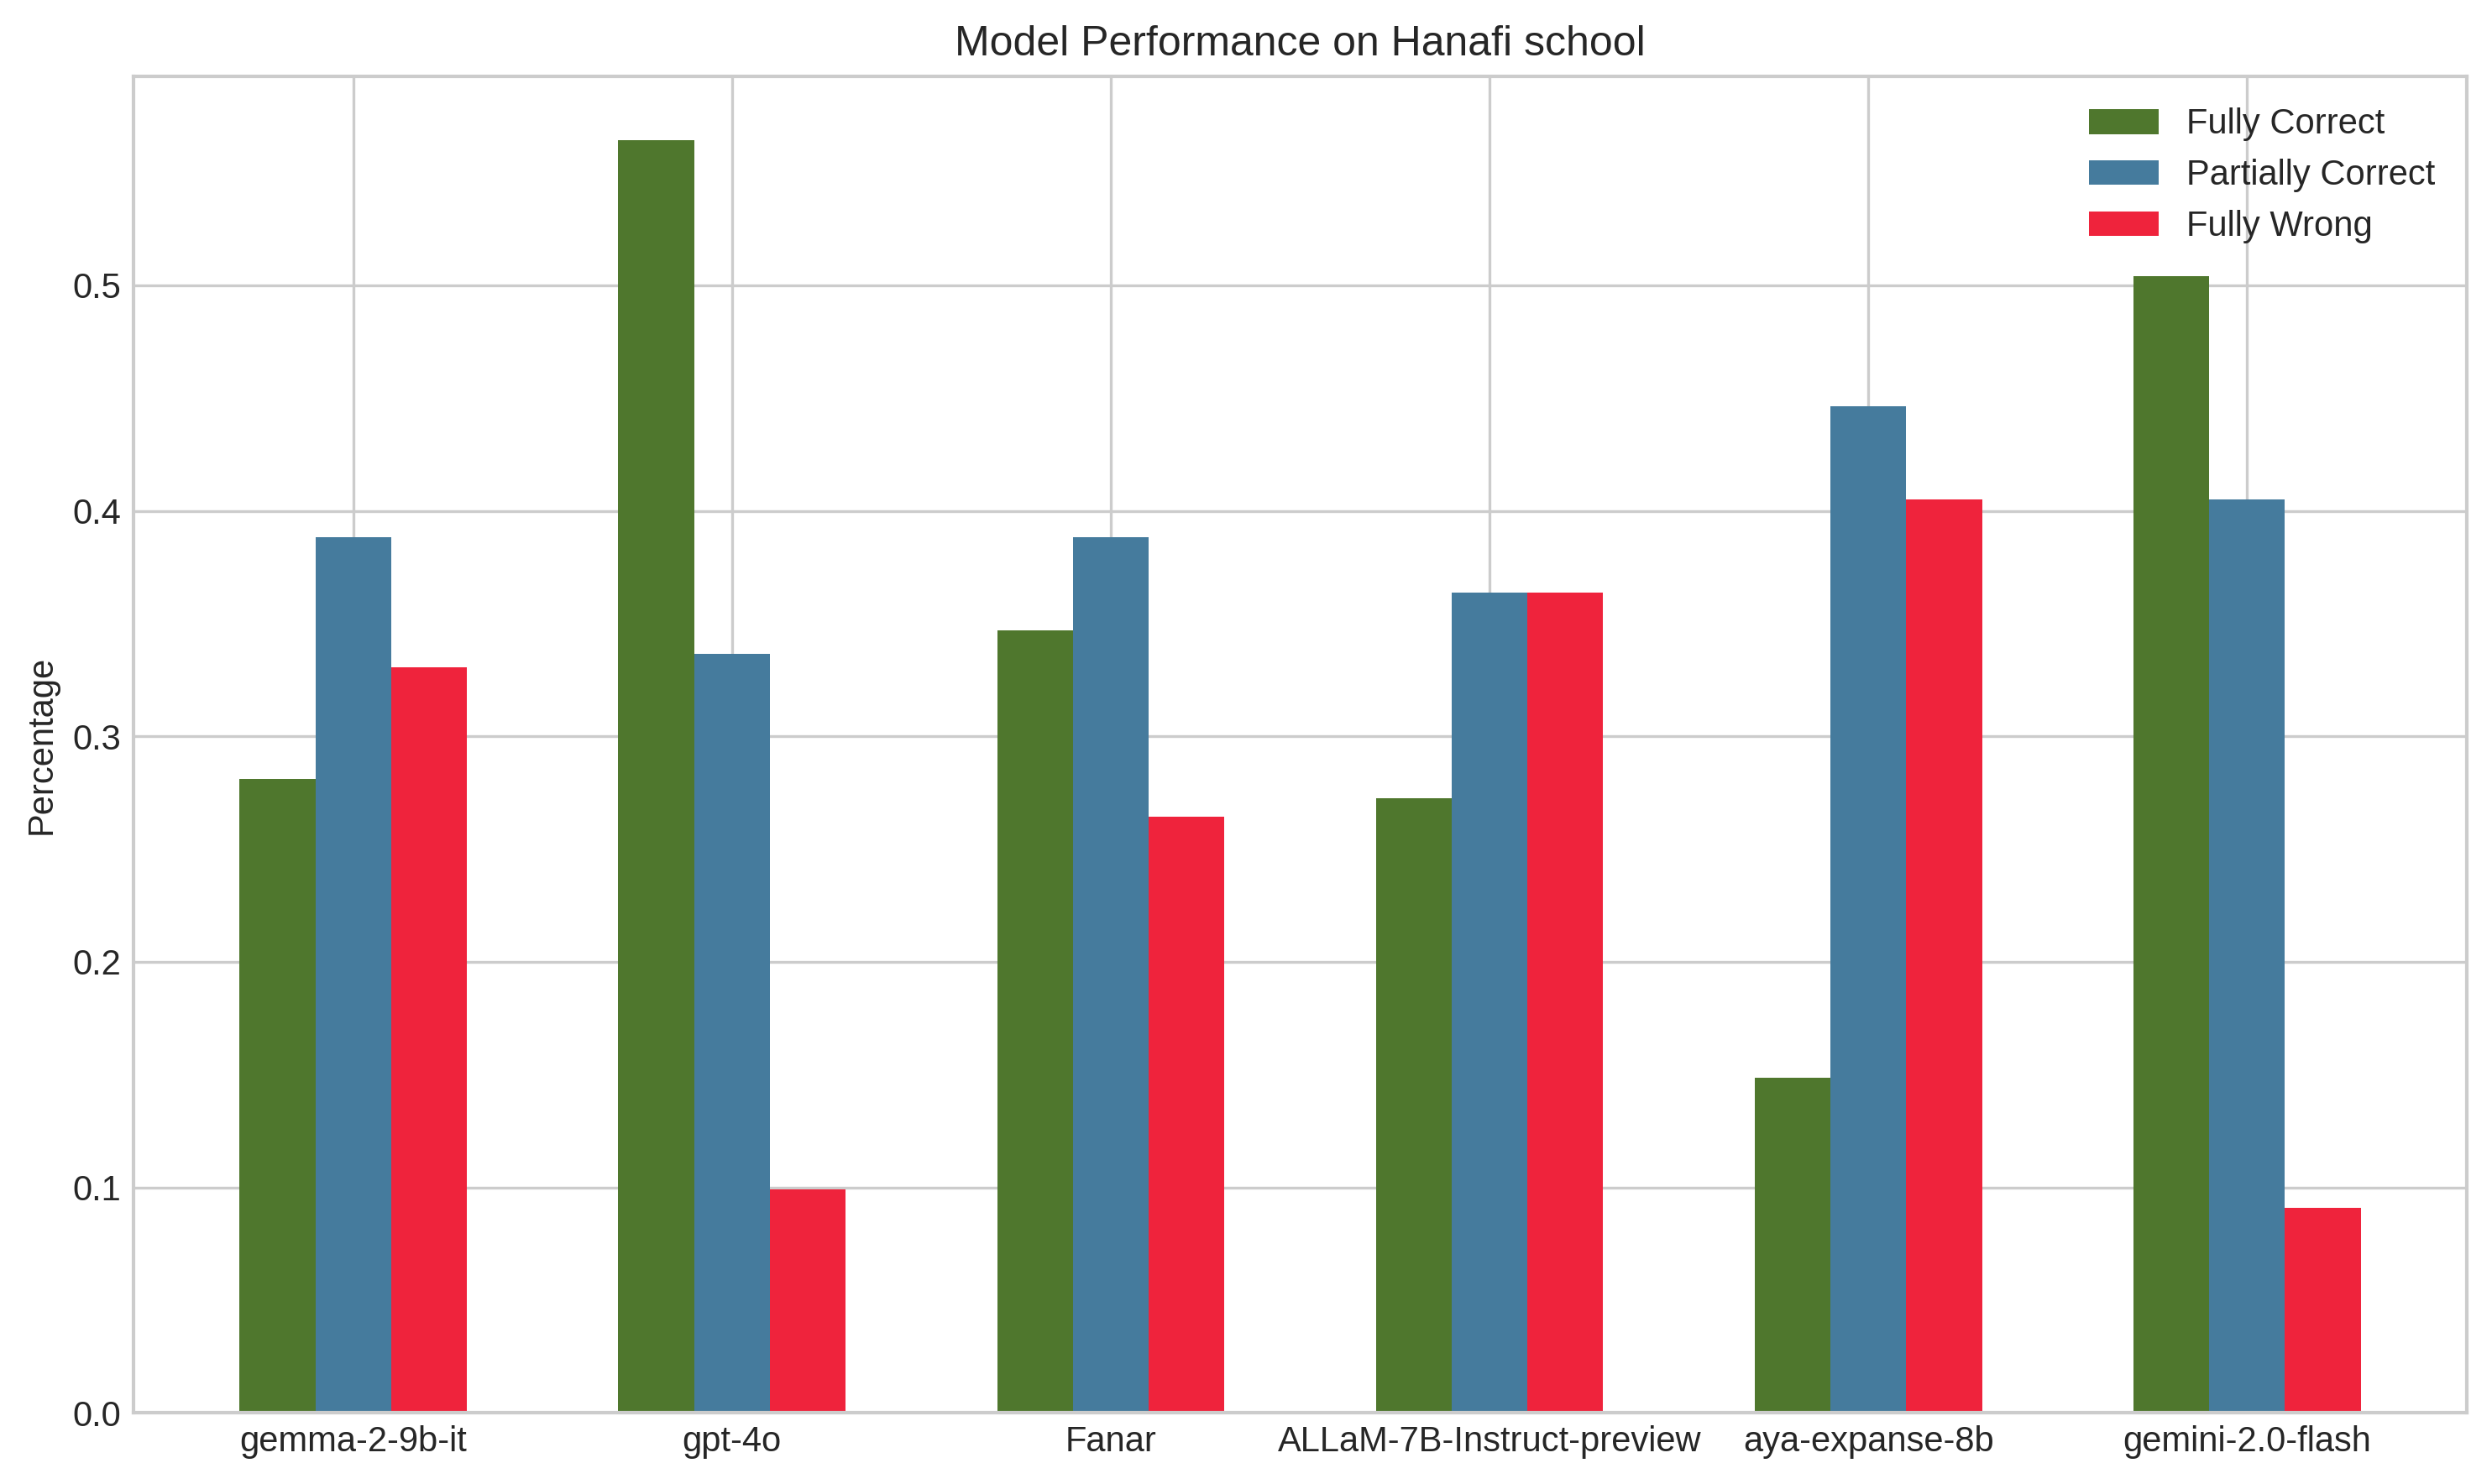
\includegraphics[height=4cm,width=0.49\linewidth]{English_Hanafi.png}
    \end{minipage}
    \caption{Model's performance on Hanafi, Hanbali, Maliki, and Shafeii schools respectively on English.}
    \label{fig:english4}
\end{figure}

\subsubsection{Basic Abstention}
Figures~\ref{fig:abst_ar} and \ref{fig:abst_en} shows the behavior of the 3 top performing models in response to the basic abstention prompts (Figure \ref{fig:mesh1}). 

\begin{figure}[h]
    \centering
    \begin{minipage}[b]{0.48\textwidth}
    \centering
    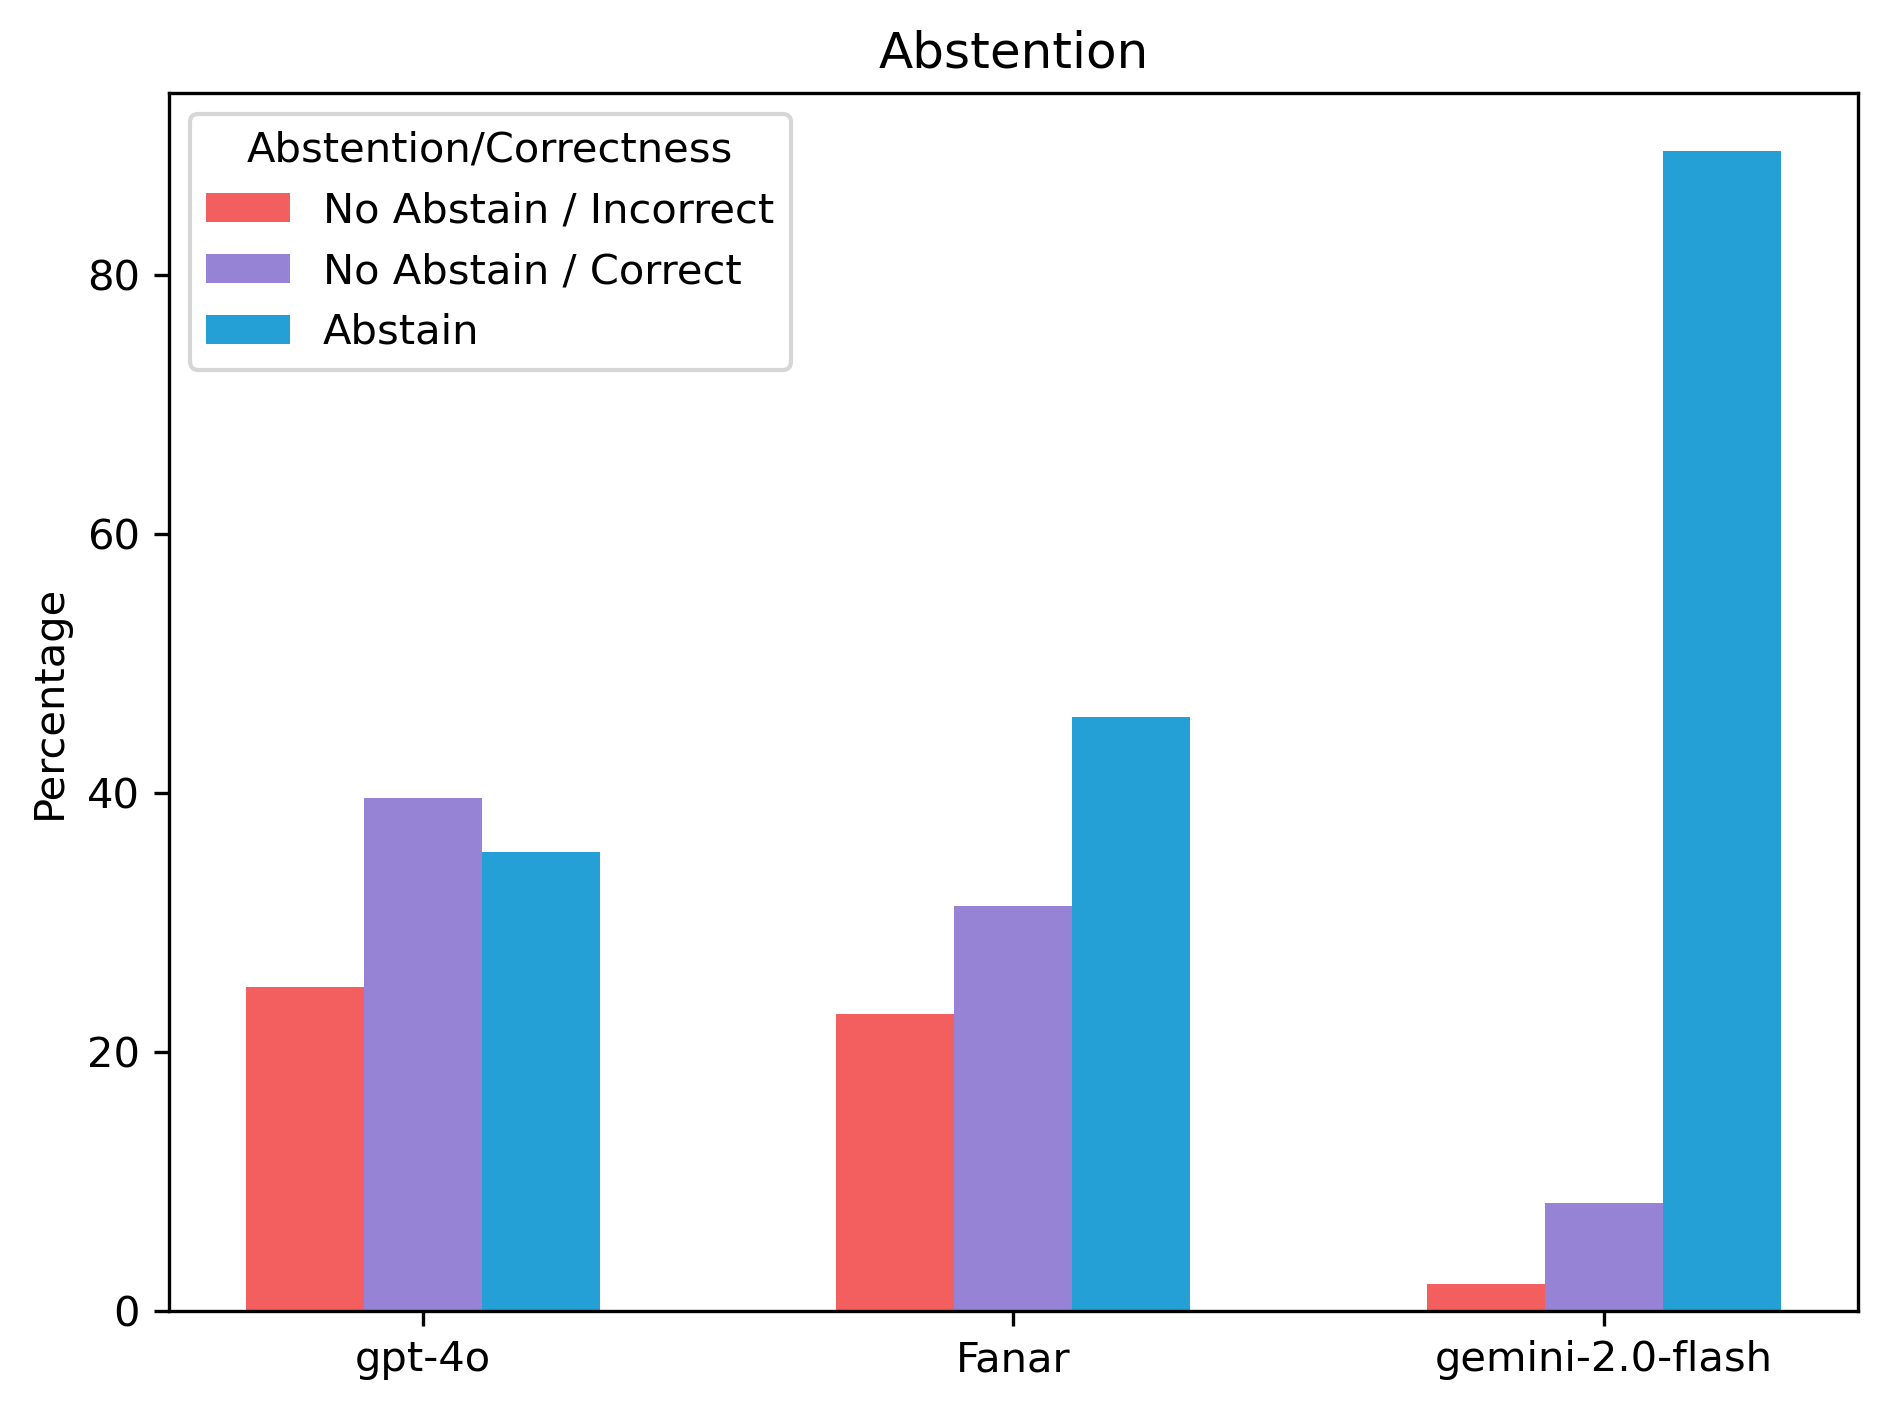
\includegraphics[width=\textwidth]{Arabic_abstention.png}
    \caption{Abstention results - Arabic QA}
    \label{fig:abst_ar}
    \end{minipage}
    \hfill
    \begin{minipage}[b]{0.48\textwidth}
    \centering
    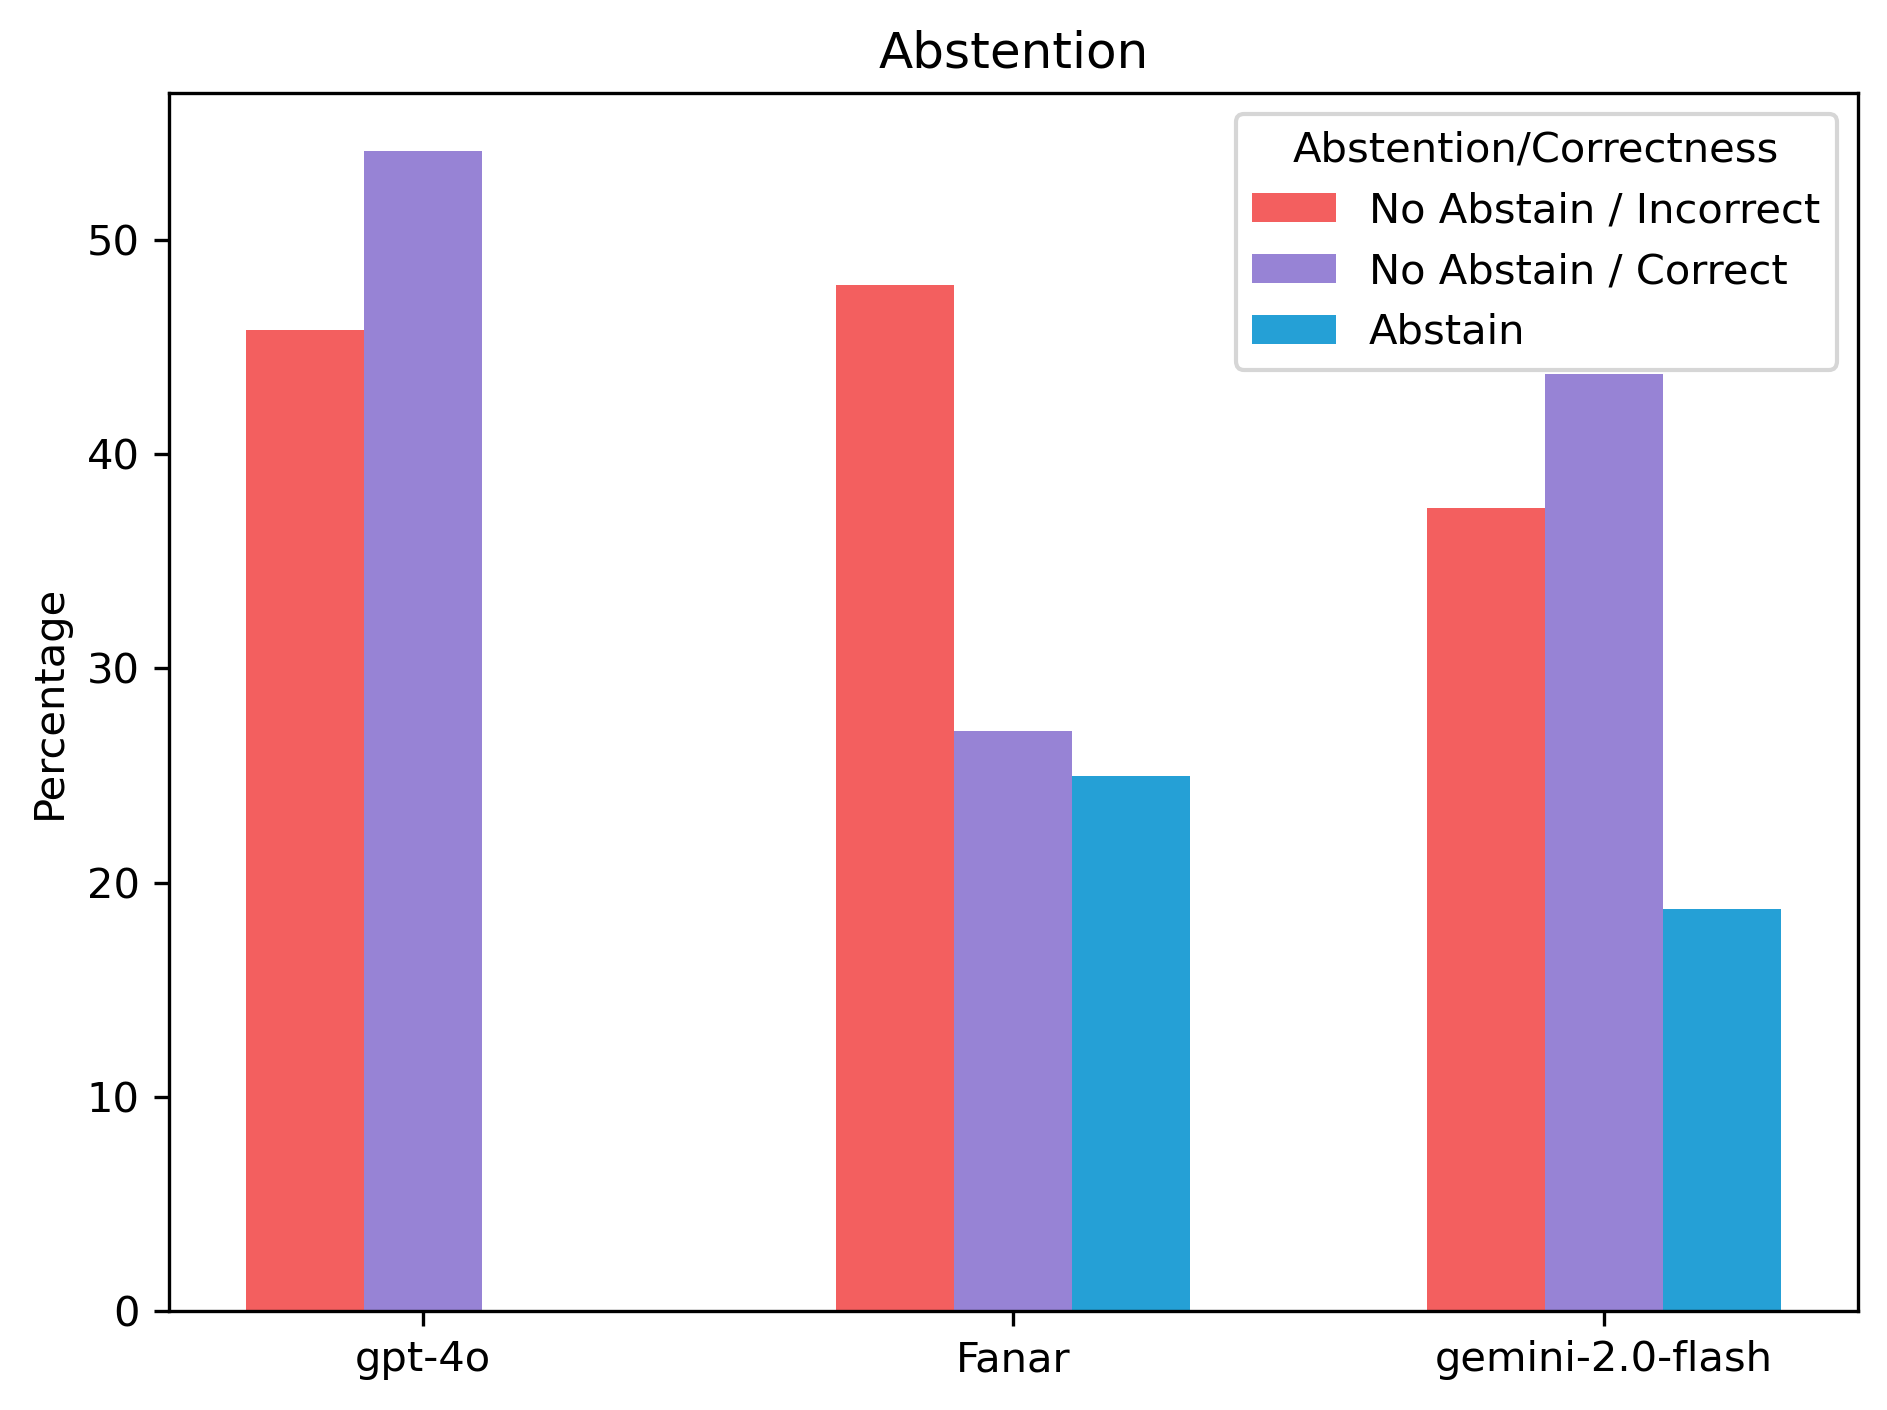
\includegraphics[width=\textwidth]{English_abstention.png}
    \caption{Abstention results - English QA}
    \label{fig:abst_en}
    \end{minipage}
\end{figure}

The behavior varies significantly on Arabic questions. Gemini exhibited the highest abstention rate, followed by Fanar and GPT-4o. Despite these abstention mechanisms, incorrect answers were still frequently generated, particularly by GPT-4o and Fanar. Notably, Gemini has an abstention rate of 90\%, with around 9\% of responses being correct and 1\% being incorrect, indicating a more conservative and reliable abstention strategy.

The behavior of the models on English data is different from Arabic. For English, GPT-4o exhibits no abstention, producing outputs for all inputs, of which approximately 56\% are correct and 45\% are incorrect. Gemini abstained in only 20\% of cases and showed a 40\% error rate alongside a 45\% accuracy rate. Fanar displayed a slightly higher abstention rate (25\%) than Gemini, but it suffers from a significantly higher error rate of 48\%.

\subsubsection{Strict abstention}

Figures~\ref{fig:strict_abst_ar} and \ref{fig:strict_abst_en} show the behavior of the LLMs with strict abstention prompts (Figure \ref{fig:mesh2}).

\begin{figure}[h]
    \centering
    \begin{minipage}[b]{0.48\textwidth}
    \centering
    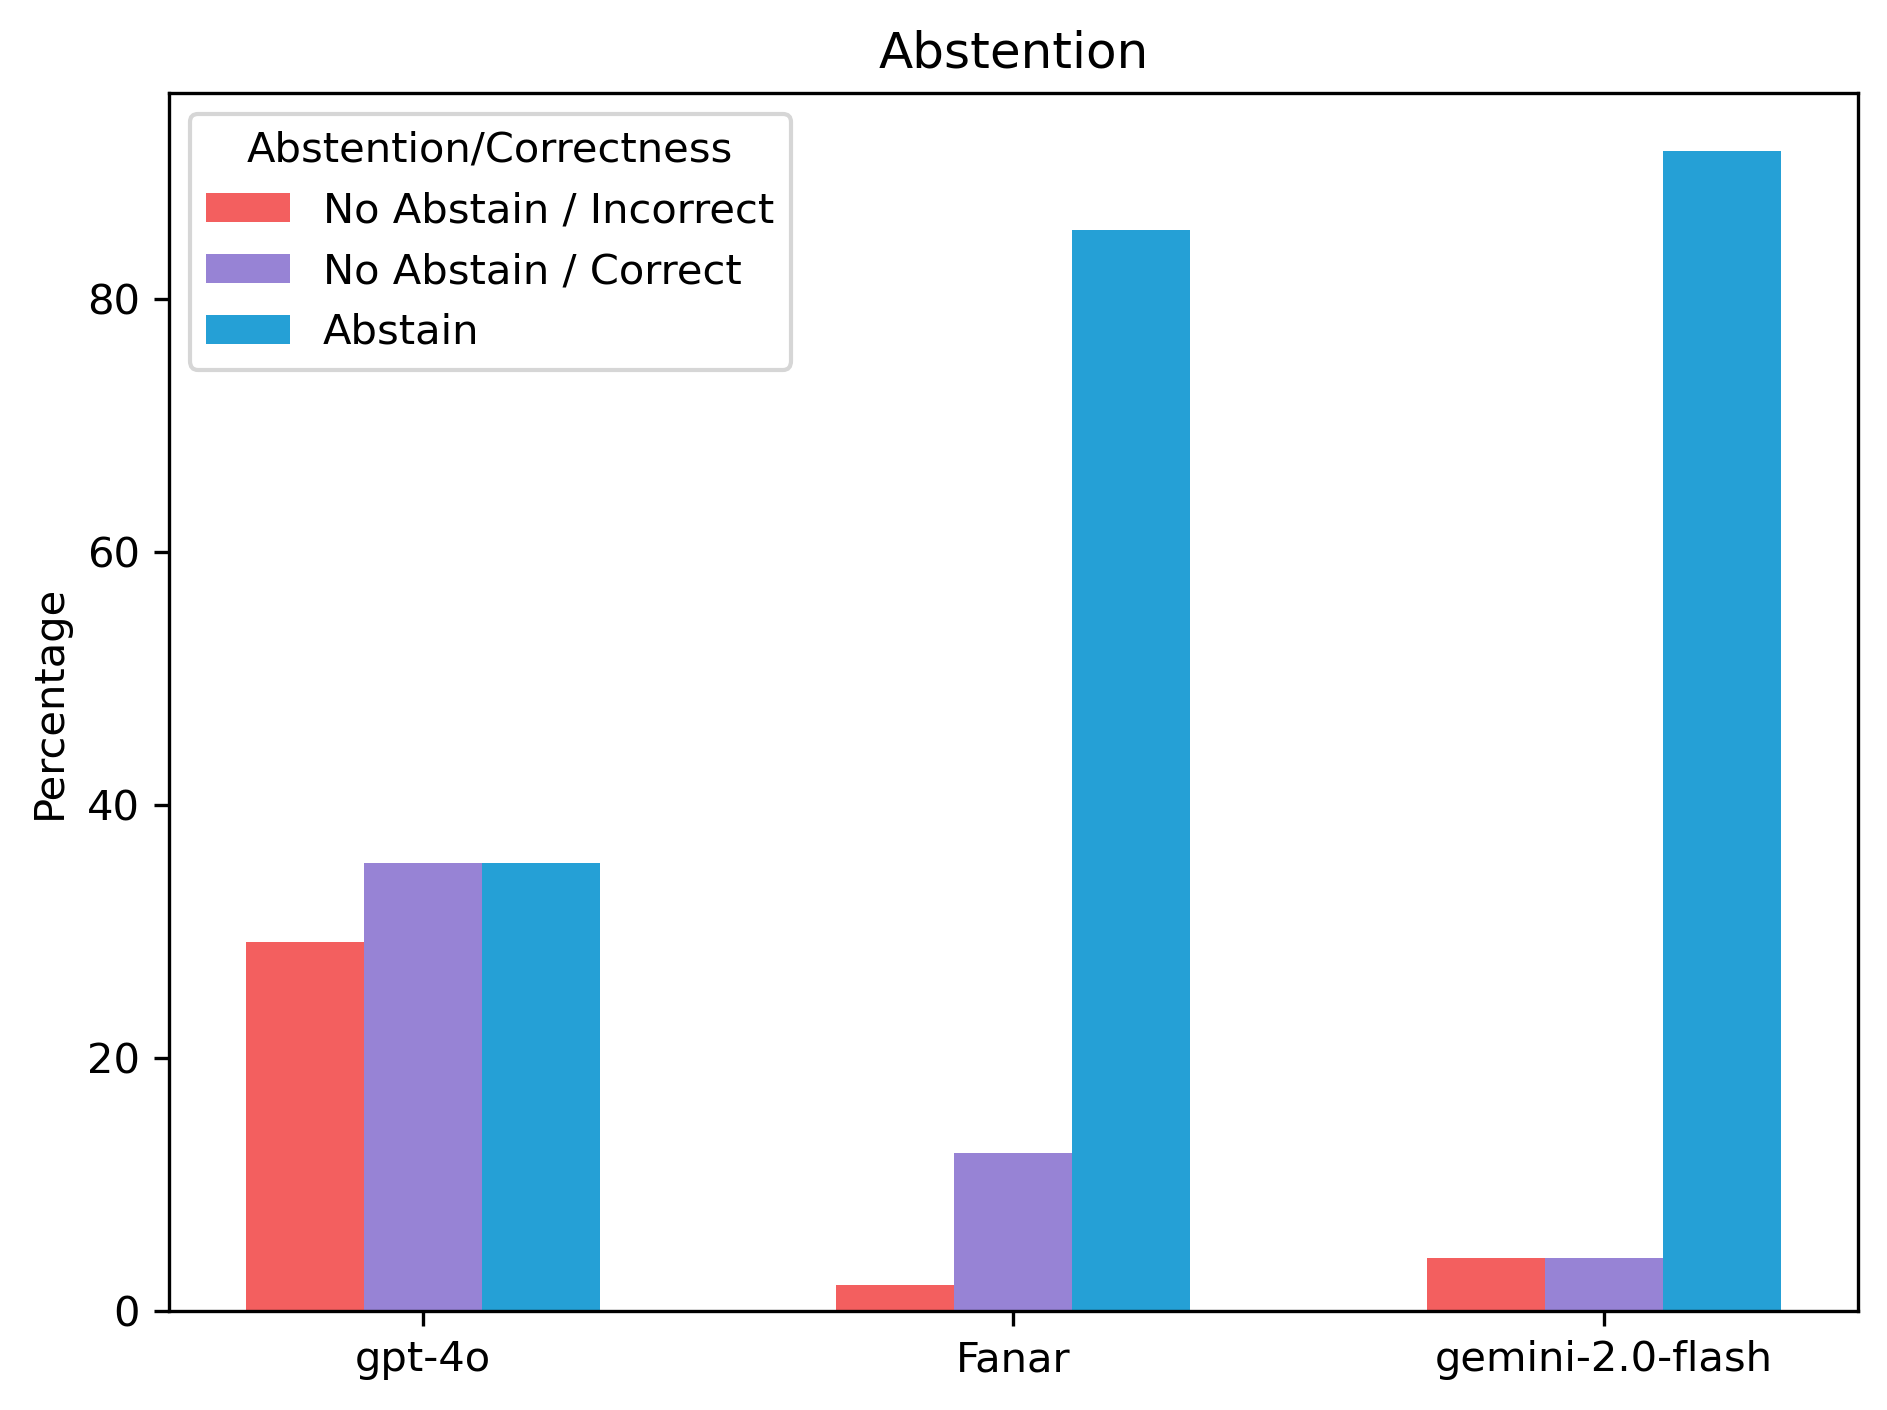
\includegraphics[width=\textwidth]{Arabic_strict_abstention.png}
    \caption{Strict abstention results - Arabic QA}
    \label{fig:strict_abst_ar}
    \end{minipage}
    \hfill
    \begin{minipage}[b]{0.48\textwidth}
    \centering
    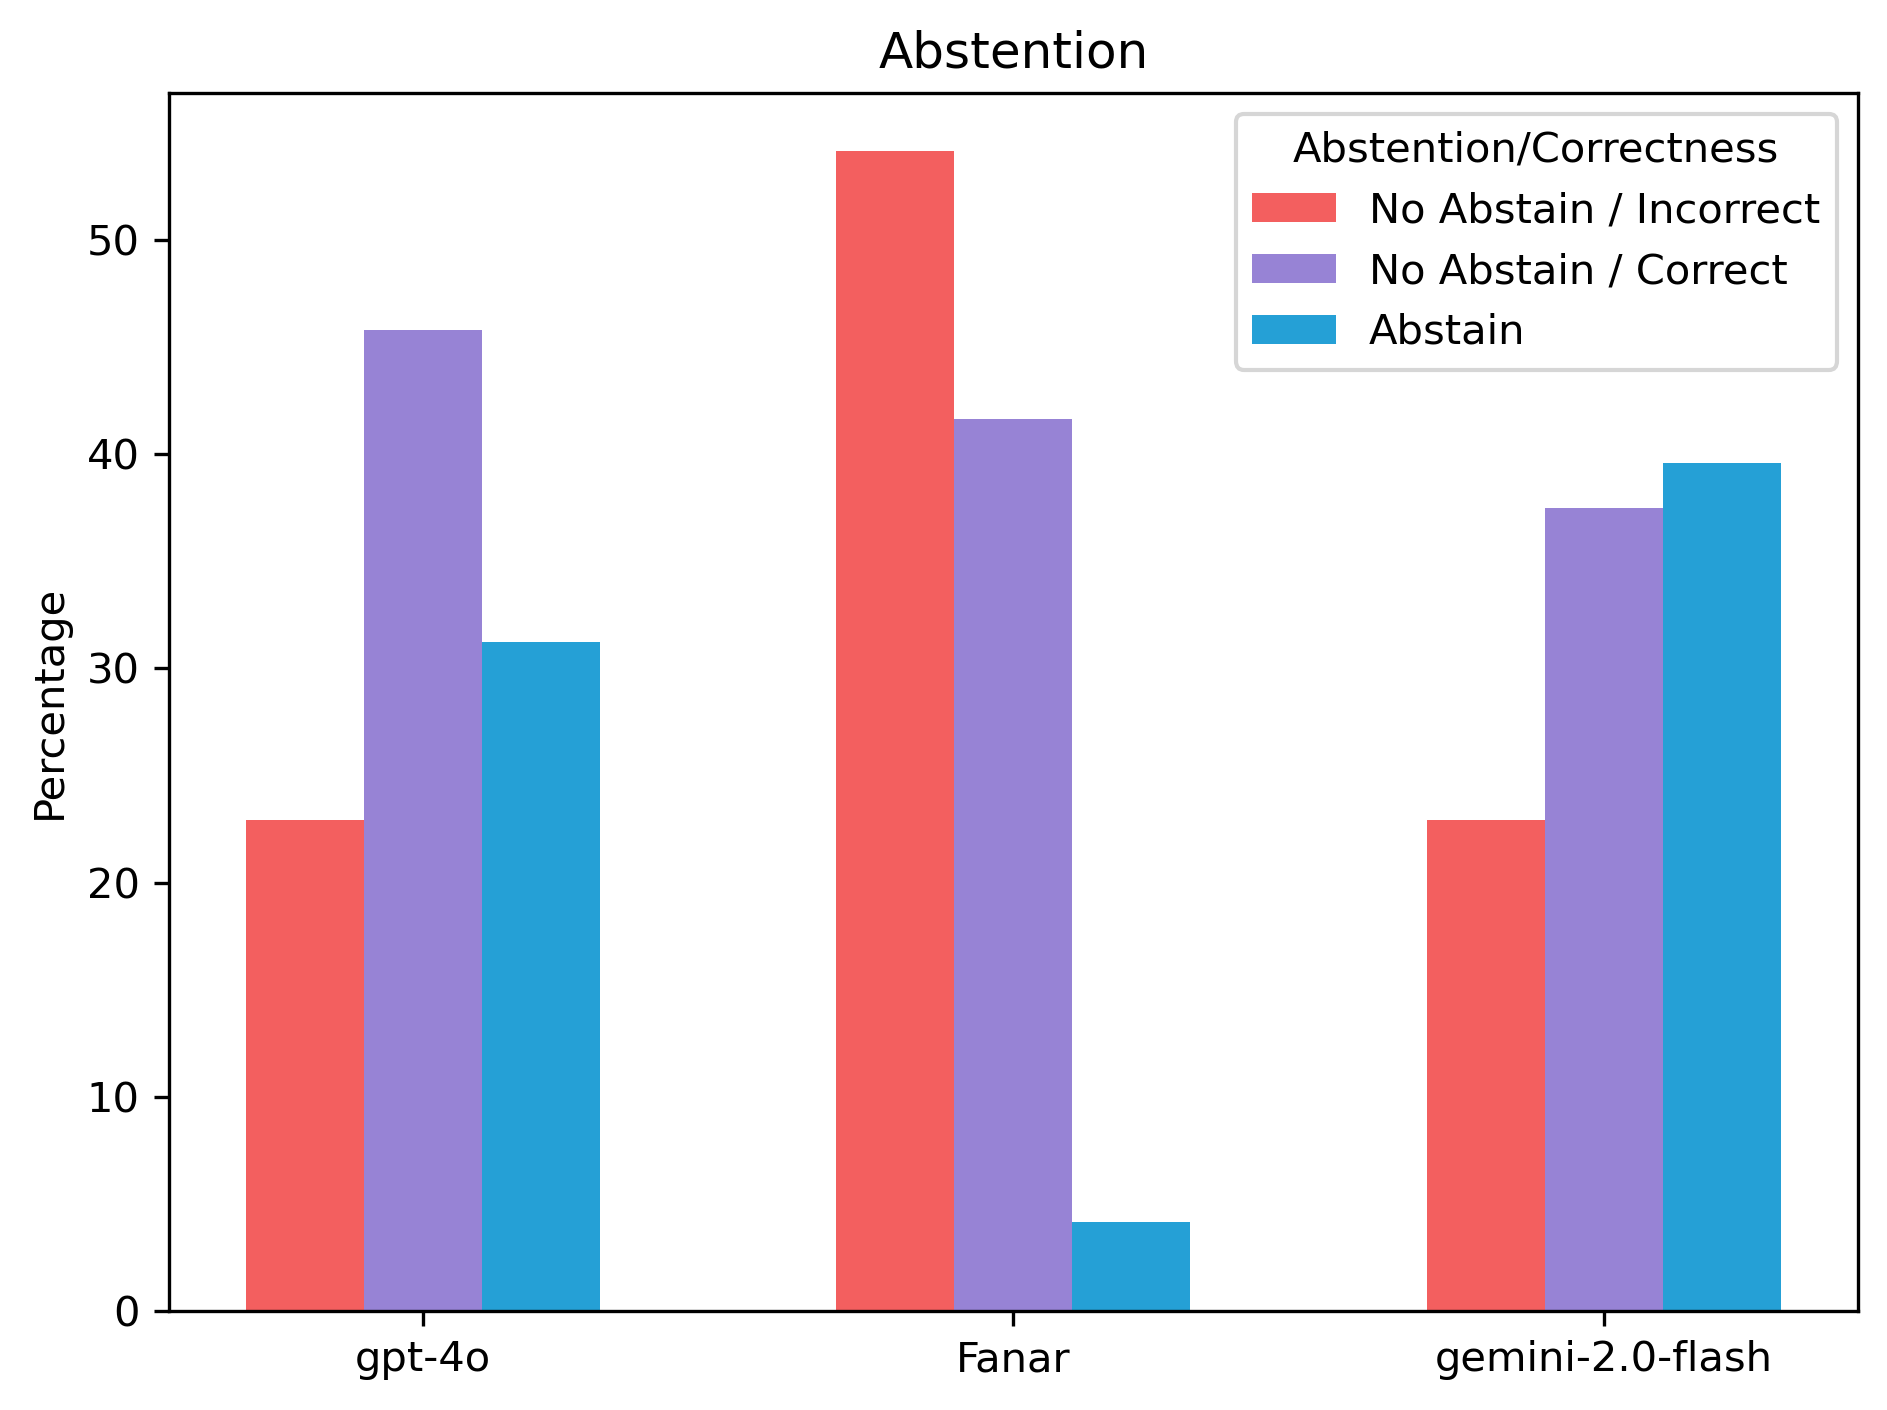
\includegraphics[width=\textwidth]{English_strict_abstention.png}
    \caption{Strict abstention results - English QA}
    \label{fig:strict_abst_en}
    \end{minipage}
\end{figure}

Under strict abstention prompting, both Fanar and Gemini demonstrated robust abstention capabilities on Arabic inputs, achieving abstention rates of 84\% and 90\%, respectively. Fanar also outperformed Gemini in terms of answer quality, with a higher proportion of correct responses and a lower error rate. GPT-4o, in comparison, abstained in only 38\% of the cases, produced a lower rate of correct answers, and produced a relatively high error rate of 30\%. Notably, GPT-4o's error rate was considerably higher than those of Fanar and Gemini under the same conditions.

As illustrated in Figure \ref{fig:strict_abst_en}, the strict abstention setting on English data revealed different trends. Gemini, followed closely by GPT-4o, showed improved abstention behavior relative to Fanar. Fanar's abstention rate remained notably low at just 4\%, coupled with a high error rate of 54\% and a correct answer rate of 42\%. GPT-4o outperformed Gemini slightly in terms of correct answers, with both models yielding comparable error rates.

\subsection{Discussion}
Our results reveal several important insights into the behavior and limitations of large language models (LLMs) in the context of Islamic question answering. First,
the zero-shot experiments show that the Hanafi school has the highest correctness rate compared to other schools for GPT-4o, while other models performed more consistently across different schools of thought. We speculate that this result is likely due to the greater availability of Hanafi-related data in public Islamic resources like IslamQA.org. This highlights an important bias in both data availability and model performance, which future work must address to ensure broader and more equitable coverage of Islamic legal traditions. Furthermore, the language gap was evident across all models, suggesting that even multilingual LLMs are significantly more reliable when responding in English, likely due to the predominance of English in pre-training corpora and evaluation frameworks. 
Third, the abstention experiments demonstrated that while GPT-4o offers strong accuracy, it is less likely to abstain when uncertain, resulting in higher rates of confidently incorrect answers. In contrast, models like Gemini and Fanar showed more conservative behavior, especially in Arabic, with higher abstention rates and lower error rates. This tradeoff between assertiveness and caution underscores a central challenge in religious AI systems: knowing when not to answer can be as important as answering correctly.

\paragraph{Persistent Reliability Challenges}
Despite improvements in abstention behavior, our findings confirm that even the best-performing models continue to produce incorrect answers. This underscores a fundamental limitation of LLMs: they are probabilistic language models, not knowledge-grounded reasoners. Each output is a sequence of tokens generated based on likelihood, not epistemic certainty. This inherent design constraint raises ongoing concerns about the reliability of LLMs in high-stakes domains such as religious rulings.

Assessing correctness remains a non-trivial task, even when the queries have known answers. Yet, a greater challenge is answering completely new questions, which require reasoning based on legal sources and principles, a process known as \emph{ijtihād}. Given the structured and rule-governed nature of both the Arabic language and Islamic jurisprudence, these domains appear fitting for computational modeling. However, realizing such a system may demand advances beyond current LLM capabilities.

\paragraph{Religious reasoning as a Human Endeavor}
It can also be argued that ijtihad is inherently a human activity, as it literally means  \textit{to strive to the utmost of one's ability}.

While AI can imitate outputs, it may be limited in replicating intention or exertion, which are key factors in the ethical evaluation of juristic reasoning in Sunni tradition. 
% The Turing test equates artificial to human intelligence based on perception and outputs, but the Islamic legal tradition also gives importance to the underlying reality of the process of how the answers were arrived at. 
According to prophetic narrations, a jurist who errs is still rewarded if a sincere effort was made\footnote{\url{https://sunnah.com/bukhari:7352}}.

Given that sincerity and effort are valued in traditional Islamic reasoning, a parallel might be drawn to the engineer or researcher developing AI systems for religious use. However, the analogy holds only if domain experts, trained scholars of law and theology, are embedded in the design and evaluation loop. The goals of the system must also align with the ethical objectives of the Islamic religion. In religious consultation, the goal is not merely to produce an answer, but to help the questioner attain benefit and avoid harm, which is the central aim of Islamic Law (\emph{Sharī'ah}).

Beyond that, valid religious reasoning requires a deep understanding of the question and its context. In complex areas such as \emph{mu'amalat} (financial and social transactions), abstaining from answering is insufficient. A competent system must identify gaps in the query and request further clarification. This requires capabilities in dialog management, contextual reasoning, and even empathy.

\paragraph{Accountability and Transparency}
When an AI system delivers an incorrect response, it is difficult to assign responsibility. Users must be cautious about delegating authority to the system, especially in religious settings. This makes transparency a moral as well as a technical imperative. It must be made explicit that the LLM outputs are probabilistic and not guaranteed to be accurate. Educating users about the limitations of such systems is essential to mitigate harm and prevent over-reliance \cite{antiquaetnova2025}.

Currently, most models offer little to no transparency about how responses are generated. Techniques such as Retrieval-Augmented Generation (RAG) and chain-of-thought prompting provide partial visibility into the reasoning process and sources. More structured dialogue flows and explicit modeling of user intent may help increase trustworthiness, but full interpretability remains a largely unsolved problem.

Our findings support a cautious and ethically grounded approach to deploying LLMs in religious contexts. Key requirements include interpretability, abstention mechanisms, context awareness, transparent reasoning, and codesign with domain experts. The goal may not be to replace human scholars but to design systems that work alongside scholars while respecting the epistemological and moral framework of the traditions they aim to serve.

\section{Conclusion}
This study presents the first benchmark specifically evaluating LLM performance in answering Islamic questions in the four major Sunni schools of thought. By introducing the FiqhQA dataset and incorporating both correctness and abstention into our evaluation, we offer a more nuanced view of model reliability in high-stakes religious contexts. While models like Gemini, GPT-4o, and Fanar show strong promise, their performance remains uneven across languages and religious traditions. Importantly, our findings underscore the need to build culturally and doctrinally sensitive systems that recognize their epistemic boundaries. Future work should focus on refining abstention mechanisms, increasing training data diversity, and improving interpretability and trustworthiness in multilingual religious domains.


\section{Limitations}

Despite following a systematic methodology in the construction and evaluation of the dataset, several limitations warrant consideration.

\subsection{Dataset Quality and Consistency}

The dataset is not without imperfections. Accurately representing the rulings of a single madhhab is already a complex task; extending this effort to cover the four Sunni madhhabs substantially increases the complexity. Although the Kuwaiti Fiqh Encyclopedia provides a comprehensive reference, the extraction and transformation of its rulings into a structured QA format required editorial interventions by the research team. In some cases, the original formulations were ambiguous or open to interpretation, requiring clarification before inclusion in the dataset.
% Additionally, all entries were translated from Arabic into English, introducing another layer where inconsistencies could arise.

The research team, being most familiar with the Hanafi school, identified and corrected several entries where inconsistencies or omissions were observed. To maintain transparency and facilitate community-based validation, the dataset will be made publicly available, and domain experts are invited to submit further corrections through the repository.

% \paragraph{Example.} An extracted ruling stated: ``It is permissible to give voluntary charity without the husband's permission.'' Upon review, the statement was refined to specify: ``It is permissible for a woman to give charity from her husband's household with his explicit permission. Additionally, giving a small amount from his wealth as charity without his permission or prohibition is also permissible.'' This clarification was necessary to align the ruling with the Hanafi school's position as documented in authoritative sources.

\subsection{Terminology Alignment Across madhhabs}

Each madhhab categorizes human actions, employing terms such as \textit{fard}, \textit{wajib}, \textit{sunnah}, \textit{mandub}, \textit{mustahab}, \textit{makrooh}, and others. These terms often have both specific and general meanings, and the same term can signify varying degrees of obligation or recommendation across different schools. For example, \textit{wajib} in the Hanafi school has a specific juristic meaning, while being an equivalent to \textit{fard} in other schools.

This complexity presents a challenge even for human scholars, and it was not explicitly accounted for in the evaluation prompts. Consequently, certain nuances were omitted in favor of a simplified evaluation scheme. Additional details on the categorization of human actions in the madhhabs can be found in publicly available resources\footnote{\url{https://islamqa.org/shafii/qibla-shafii/33285/categories-of-human-actions/}, \url{https://www.islamandihsan.com/mandub-maliki}}.

\subsection{Variability in Question and Answer Interpretation}

The open-ended nature of the questions results in variability in how the LLM interprets and answers them. In some cases, the LLM’s understanding of the question differs from the expected interpretation, though the response may remain plausible within the domain. This discrepancy can complicate the evaluation process. Moreover, the formulation of the answer itself impacts the rating. Ideally, answers should be clear and unambiguous. 

% For example: ``It is permissible for a woman to give charity from her husband's household with his explicit permission. Additionally, giving a small amount from his wealth as charity without his permission or prohibition is also permissible.'' Such specificity aids in accurate evaluation.

Another observed behavior is that LLMs often provide additional information beyond the scope of the question. While this mirrors practical fatwa-giving behavior, it introduces complexity in evaluation. In our framework, providing extra relevant information may result in a rating of 2 (partial correctness), although it may be argued that such comprehensive answers should be rated as fully correct. This remains an open consideration.

% \subsection{Scope of Opinions Required}

% A key consideration in evaluation is whether the LLM should provide all recognized opinions within a madhhab or whether presenting the dominant opinion suffices. In this study, the LLM was prompted to include all opinions where applicable. Nevertheless, this approach introduces challenges, as it may not always align with the expectations of lay users, for whom the main opinion is often sufficient.

% \paragraph{Example.} In the Hanbali school, \textit{Al-Muwalat} in ablution is considered obligatory. However, there exists a minor narration within the school that regards it as recommended (sunnah). An LLM response that mentions only the minor opinion without acknowledging the obligatory ruling results in a rating of 2. If the LLM correctly identifies the obligatory ruling, it is rated as 3.

% \subsection{Prohibition Bias in Model Responses}

% An observed hypothesis during evaluation was that when the LLM is uncertain or lacks knowledge, it tends to err on the side of prohibition. This conservative bias results in responses that default to prohibiting an action when the correct ruling is permissibility or recommendation. This may lead to systematic inaccuracies in the dataset.




% Entries for the entire Anthology, followed by custom entries
\bibliography{aaai25}

% \newpage

% \begin{appendices}
% \chapter{Appendix A: Prompts}



% \end{appendices}
\end{document}

